\documentclass[runningheads]{llncs}
%
\usepackage{graphicx}
\usepackage{subcaption}
\usepackage{hyperref}
\usepackage{float}

\begin{document}
%
\title{PhageScan - Automated viral particle detection}
%
\titlerunning{PhageScan}
%
\author{Sousa, R.\inst{1}\orcidID{0009-0000-2558-7176} \and
Dias, O.\inst{1}\orcidID{0000-0002-1765-7178} \and
Oliveira, H.\inst{1}\orcidID{0000-0001-9564-5714}}
%
\authorrunning{Sousa et al.}
%
\institute{Department of Biological Engineering, University of Minho, Campus de Gualtar, 4710-057, Braga, Portugal \email{sac@ceb.uminho.pt}\\
\url{https://www.deb.uminho.pt/} }
%
\maketitle              % typeset the header of the contribution
%
\begin{abstract} 

Bacteriophages are viewed as a promising solution to fight antibiotic-resistant bacteria. Being the most abundant organism in the biosphere, classifying these viruses is a complex and morose task that can be obviated through application of computational tools. This work proposes PhageScan, a tool to identify phages from Transmission Electron Microscopy images using YOLO algorithms. In this first iteration we have achieved a model capable of identifying siphoviruses with relative precision for a confidence threshold of around 0.4, with a large margin for improvement.

\keywords{Bacteriophage classification \and deep learning \and convolutional neural networks}
\end{abstract}
%
%
%
\section{Background}
%
%
\subsection{
What are bacteriophages?}

Bacteriophages (phages), regarded the most abundant organisms in the biosphere, are a type of virus that thrives by infecting and replicating within bacterial cells. \cite{batinovic2019} These organisms are generally species-specific, typically targeting a single bacterial species to maintain their lifecycle and co-evolving with it. \cite{clokie2011,kasman2022,koskella2014,suttle2005}
%
%

Phages adopt two distinct life styles: lytic or lysogenic (Fig~\ref{fig1} \cite{varona2017}). Lytic phages infect the host cell and hijack its biosynthetic machinery to rapidly generate offspring that exit the cell, bursting and killing it in the process. Phages with a lysogenic life style, by their turn, can be stable for generations, integrating their genome in the host's, sometimes even shaping the host phenotype. In this state, they do not necessarily kill the host, adopting an opportunistic approach, transitioning towards a lytic approach when the host reaches its end of life and / or if a specific trigger occurs. There are also phages that exhibit a a chronic life style, which is generally non-bactericidal. \cite{clokie2011,varona2017,ioannou2023}

\begin{figure}
\begin{center}
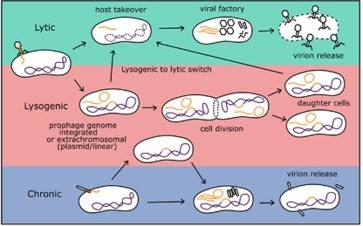
\includegraphics[width=0.4\textwidth]{./figures/fig1-lifecycle.jpg}
\caption{Simple schematic representation of the different phage life cycles. \cite{varona2017}} \label{fig1}
\end{center}
\end{figure}

Given their natural predating relationship with bacteria, phages are increasingly gaining traction as potential therapeutic agents in the combat of antibiotic-resistant bacteria, a pressing global health challenge.\cite{ioannou2023,haq2012,gamachu2022,sulakvelidze2001}
%
%
A result of this growing interest in phages creates a pressing need to develop methods to study phages to facilitate identification and classification. 

\subsection{Phage classification}
With the advancements in genomics and metavirunomics, phage classification underwent significant changes in recent years, transitioning from a morphological to a genomically coherent taxonomical method. The biggest change in the system was abolishment of the most abundant family of phages, caudovirales (Fig~\ref{fig2} \cite{dion2020}), which was divided into three subfamilies: (i) Podoviridae; (ii) Myoviridae; and (iii) Siphoviridae. In its stead emerged the new class of caudiviricetes, comprised of 4 new orders and 22 new families. \cite{dion2020,turner2021,turner2023,ackermann2007}   
%
%
\begin{figure}
\begin{center}
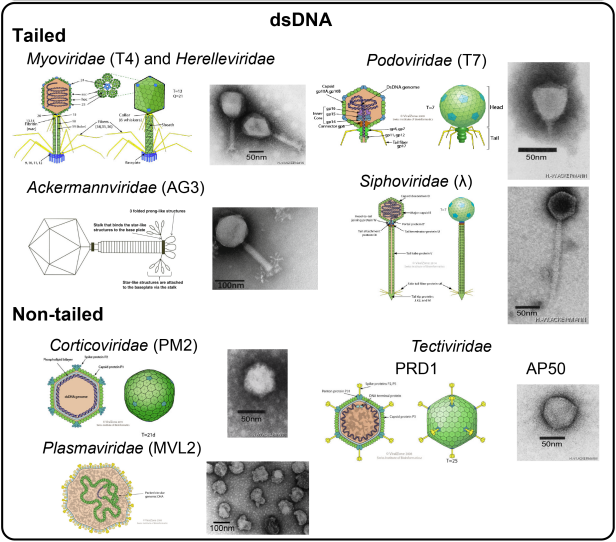
\includegraphics[width=0.4\textwidth]{./figures/fig2-tailed-morpho.png}
\caption{Schematic representation of tailed phages morphology. \cite{dion2020}} \label{fig2}
\end{center}
\end{figure}

%
%
Despite morphology no longer being used, it remains relevant towards identification and classification, standing out as a potential approach for automating tailed phage classification from Transmission Electron Microscopy (TEM) images. There are three distinct tailed phage morphotypes (Fig~\ref{fig3}), based on their respective tailed structures: podoviruses, siphoviruses and myoviruses. \cite{maffei2021} \textbf{Podoviruses} typically display a short non-contractile tail and an icosahedral capsid of about 60 nm in diameter. An example of this virus is \textit{Brucealvirus} CP7R as shown below. \cite{volozhantsev2012} \textbf{Siphoviruses} typically display an icosahedral capsid and a long, flexible but non-contractile tail, spiked at the tip. An example of this morphotype, BlueFeather, can be seen below. \cite{demo2021} \textbf{Myoviruses} display a contractile tail with a base plate and spikes at the tip and an icosahedral capsid. One example of this viruses is \textit{Synechococcus} Phage S-PM2. \cite{mann2005}

\begin{figure}
    \begin{center}
        
    
    \begin{subfigure}[b]{0.2\textwidth}
        \begin{center}
        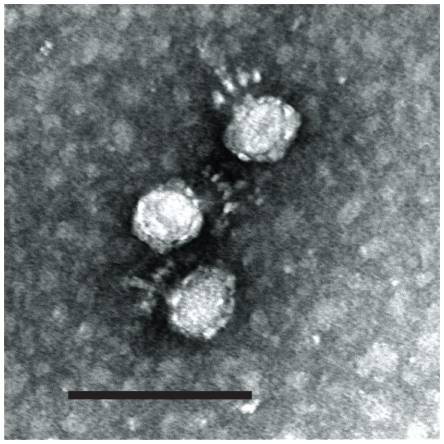
\includegraphics[height = 75px]{./figures/fig-3-1-podovirus.jpg}
        \caption{Podovirus}
        \end{center}
    \end{subfigure}
    %\hfill
    \begin{subfigure}[b]{0.2\textwidth}
    \begin{center}
        
    
        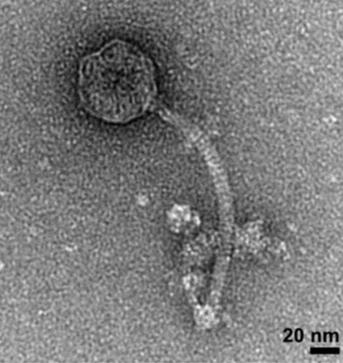
\includegraphics[height = 75px]{./figures/fig-3-2-siphovirus.jpeg}
        \caption{Siphovirus}
        \end{center}
    \end{subfigure}
    %\hfill
    \begin{subfigure}[b]{0.2\textwidth}
    \begin{center}
        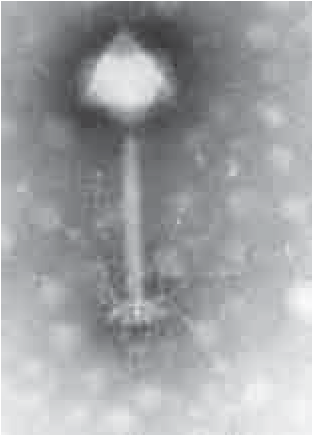
\includegraphics[height = 75px]{./figures/fig-3-3-myovirus.png}
        \caption{Myovirus}
        \end{center}
    \end{subfigure}
    \caption{Morphotypes of phages present in the caudoviricetes class, the most abundant class of phages in the currently existing knowledge. From left to right are shown specimens of podovirus CP7R, a \textit{Chlostridium perfringens} phage, siphovirus BlueFeather, a \textit{Arthrobacter globiformis} phage, and myovirus S-PM2, a \textit{Synecochus sp.} phage. \cite{volozhantsev2012,demo2021,mann2005}}
    \label{fig3}
    \end{center}
\end{figure}


\subsection{Automated viral particle detection and classification}

One of the main advantages of developing accurate and efficient methods for automatic detection of viral particles is the automation of the fastidious and labour-intensive work associated with microscope analysis - safeguarding the impact that human factors such as fatigue can have on the analysis.  \cite{glaeser2004}  This is also the case for automatic recognition of viral particles, where qualitative and quantitative measurements involve processing of thousands of microscopy images to count particles and identify viral morphotypes. \cite{glaeser2004,gelzinis2015}

It is accepted that in order to be regarded as valuable, automatic recognition systems must attain an accuracy greater than 75\% when compared to a human expert. \cite{glaeser2004} There are several methods in the literature for automatic particle identification using machine learning techniques  such as neural networks, Gaussian classifiers, Naive Bayes, and random forests that have achieved this requisite to different degrees. \cite{gelzinis2015,ogura2004,sorzano2009,castanon2007} From these methods, we highlight neural networks, specificall convolutional neural networks (CNNs) as particularly adequate for the purpose of automated phage classification given their specialization in processing grid-like data. 

\subsection{An overview of CNNs}

CNNs are a variation of Neural Networks, consisting of a feed forward mathematical model that contain: i) an input layer; ii) N hidden layers each containing M number of neurons that perform mathematical operations for classification; iii) and output layer representing the outcome of said calculations, usually the classification of the input under the form of a probability. This is achieved due to neurons having distinct weights (W) and biases (b), thus influencing the classification process. \cite{teuwen2020} A neuron can be represented mathematically as an affine function followed by a non-linearity: 

\begin{equation} \label{eq1}
    M(x) = \phi \cdot (W \cdot x + b)
\end{equation}

CNNs have emerged as an approach to process grid-like data, such as images, adopting a sweeping approach, enabling weight sharing and local neuron responses instead of activating all the neurons of the network thus enhancing its efficiency. Conversely, CNNs are also constituted by convolutional layers and pooling layers.

\subsubsection{Convolutional layers} operate on the input data (\textit{i.e.} image) using vector and matrix operations in order to extract features from input data, generating a feature map. The mathematical operation performed by the convolutional layers is called a convolution and can be represented mathematically by

\begin{equation} \label{eq2}
    (x \cdot w)(a) = \int x(t) \cdot w(a – t) d \cdot a
\end{equation}

Where $a$ is an n-dimensional vector that iterates over all values in the input, $w$ represents the convolutional kernel, a matricial filter or mask that operates and transforms the data. The integral is replaced by the higher dimensional variant of $a$. In the context of this work we will only use 2D microscopy images and as such will be working with 2-dimensional convolutions, which can be represented mathematically by

\begin{equation}
    (I \cdot K)(i,j) = \sum_{m} \sum_{n}(I(m,n)K(i-m,j-n)
\end{equation}

\subsubsection{Pooling layers} act as intermediate nodes, performing dimensionality reduction and downsampling operations to the feature map while retaining essential features.  

Each operation is followed by the application of an activation function which adds non-linearity to the system, aiding in the classification of the input.There are several activation functions, but for the sake of this work, we'll detail SiLU (Sigmoid-Weighted Linear Units), which is the activation function we will be using during the training \href{https://blog.roboflow.com/a-thorough-breakdown-of-yolov4/}{of YOLOv8} \cite{teuwen2020}.

SiLU delivers smooth profiles by combining linear and non-linear functions, thus increasing feature detection sensitivity. SiLU can be represented mathematically as:

\begin{equation}
    SiLU(x) = x \cdot \sigma(x)
\end{equation}

where $\sigma(x)$ is the sigmoid function given by:

\begin{equation}
    \sigma(x) = \frac{1}{1 + e^{-x}}
\end{equation}

and $x$ is the input \cite{elfwing2018}.

\subsubsection{Finally, fully connected layers} or dense layers take in the output of the previous layers and flattens it, transforming the representation of all feature maps into a single vector. The final fully connected layer is the output layer that gives the final probabilities for each considered class.  Figure \ref{fig4} depicts the architecture of a CNN. \cite{Alzubaidi2021}


\begin{figure}
\begin{center}
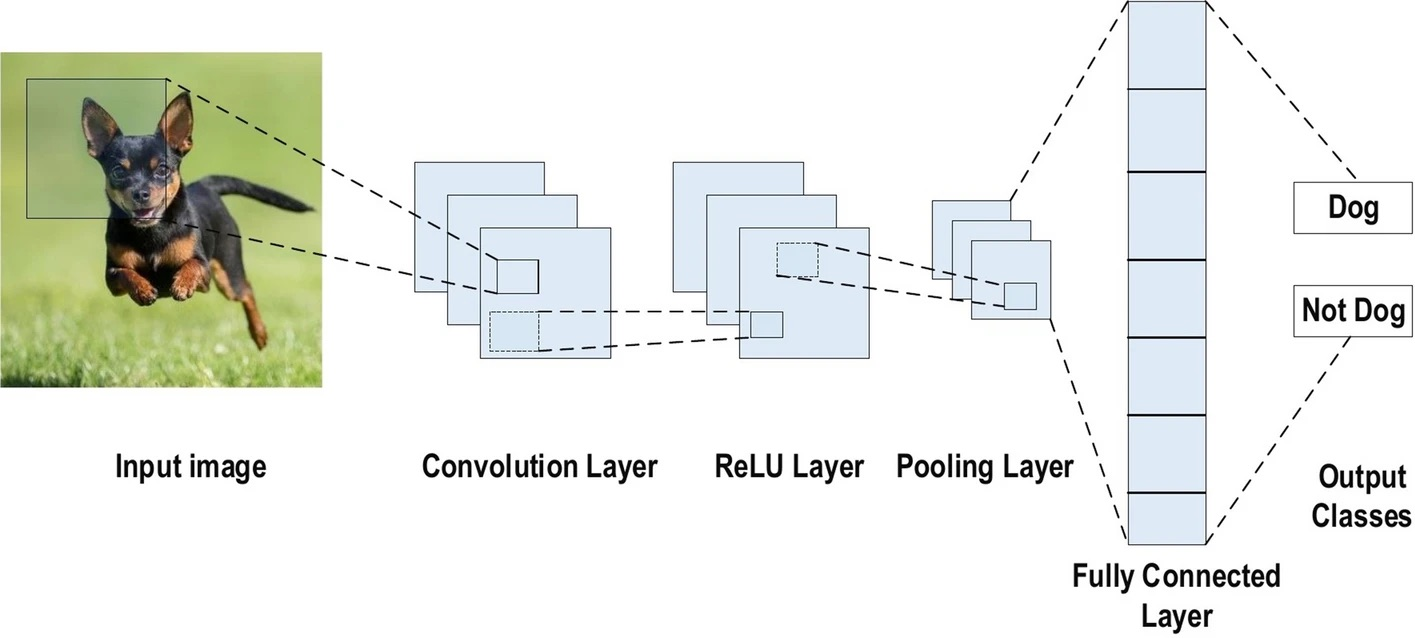
\includegraphics[width=.5\textwidth]{./figures/fig-4-cnn_repr.jpeg}
\caption{Schematic representation of a CNN. \cite{Alzubaidi2021}} \label{fig4}
\end{center}
\end{figure}


\section{Methods/approach}

This work aimed to explore and evaluate the employment of CNNs in automated phage particle recognition given their versatility and high level of discernment for image classification with high accuracy. \cite{ogura2004} Moreover,  we explored and evaluated the application of \href{https://docs.ultralytics.com/models/yolov8/}{You Only Look Once (YOLO)} algorithms, specifically YOLOv8. YOLO was created as an approach for object detection and has been demonstrating growing accuracy and real-time performance and have already been employed in the field of biological images processing. \cite{li2023,zhu2023,gonzalez2023}

It is important to consider several challenges that this project entails, including: (i) the lack of publicly available data sets, (ii) high noise levels in available TEM micrographs, (iii) a lack of variety of phages and hosts on a sample, (iv) podoviruses have small tails that can be difficult to detect, possibly being confounded with vesicles, and myoviruses have contracted/relaxated tails, adding complexity to labeling and classification as they can be confounded with siphoviruses, (v) recently the first-ever observation of phages attaching to another viruses was made, further adding complexity to this task \cite{deCarvalho2023}. Considering these challenges, siphoviruses, with their consistent capsid shape and long non-contractile tails, are a good starting point and, in future steps, the application of more complex image processing techniques, such as edge detection/filtering and pixel intensity interpolation, are needed. 

\subsection{Data set creation}

\subsubsection{Data gathering and pre-processing}

The data set was created through sourcing 119 siphoviruses TEM micrographs from \href{https://phagesdb.org/} and {PhagesDB} together with TEM images obtained from the CEB-UMINHO phage research lab.

The data was pre-processed by: i) resizing images to a fixed size (640 x 640 pixels), ensuring all scales are correctly represented; ii) adjusting image quality (brightness, contrast, noise and artifact removal).

\subsubsection{Annotation}
Finally, to make the data set processable by the model, it’s fundamental to annotate the images in order to specify what is what. This process is achieved through specifying object classes and location within the images with bounding boxes. The data set images were anottated using \href{https://docs.ultralytics.com/integrations/roboflow/}{Roboflow}. The annotation process for phages followed the following approach: (i) draw a bounding box directly on top of the phage, classifying phages in micrographs where there are other objects present, increasing context in micrographs where could exist other objects with strong contrast resembling the head such as bacteria.

\subsubsection{Augmentation}
The data set will be augmented through \href{https://blog.roboflow.com/why-and-how-to-implement-random-rotate-data-augmentation/}{random rotations and flips} in order to create scenarios where the target objects of classification and identification can be identified independently from image rotation angle, being this a common data augmentation approach for object detection algorithms. \cite{gonzalez2023} 

\subsection{Training parameters}
The training was performed using YOLOv8, on each pass through the data set (epoch) the data set was subdivided in batches of 16 images. The data set contained 271 images, corresponding to approximately 17 batches. The model was trained for 10/25/50 epochs corresponding to 170/425/850 optimization steps respectively, using SiLU activation function and a training rate of 10e-3 (Adam). 

\section{Results}

In this section, we analyze and compare the performance metrics of various trained models, focusing on box, class, and distribution focal losses, as well as precision, recall, and F1 score.

\subsection{Training Results - 10 Epochs}

Figure \ref{fig5} illustrates the training outcomes for the model trained over 10 epochs. Analyzing these results reveals a consistent improvement across the epochs, with a notable decline in box, class, and distribution focal losses (DFL) for both training and validation sets. This trend indicates an enhanced model capability in inferring and identifying correct bounding box coordinates, class attributions, and discerning underrepresented classes, specifically distinguishing between siphoviruses and the background.

Moreover, despite the decreasing trend in these metrics, they have not yet reached a plateau, suggesting that further training could yield additional improvements. This potential for enhancement is further corroborated by a continuous increase in the model's precision, average precision at a confidence threshold of 0.5, average precision across the range of 0.5-0.95, and recall. These improvements indicate that the model is progressively better at correctly identifying true instances of objects and assigning the appropriate class.

The consistent upward trend in these performance metrics, coupled with the absence of plateau behavior, strongly suggests that the model's performance could be further enhanced with additional training epochs, as will be demonstrated in subsequent sections.

\begin{figure}[H]
\begin{center}
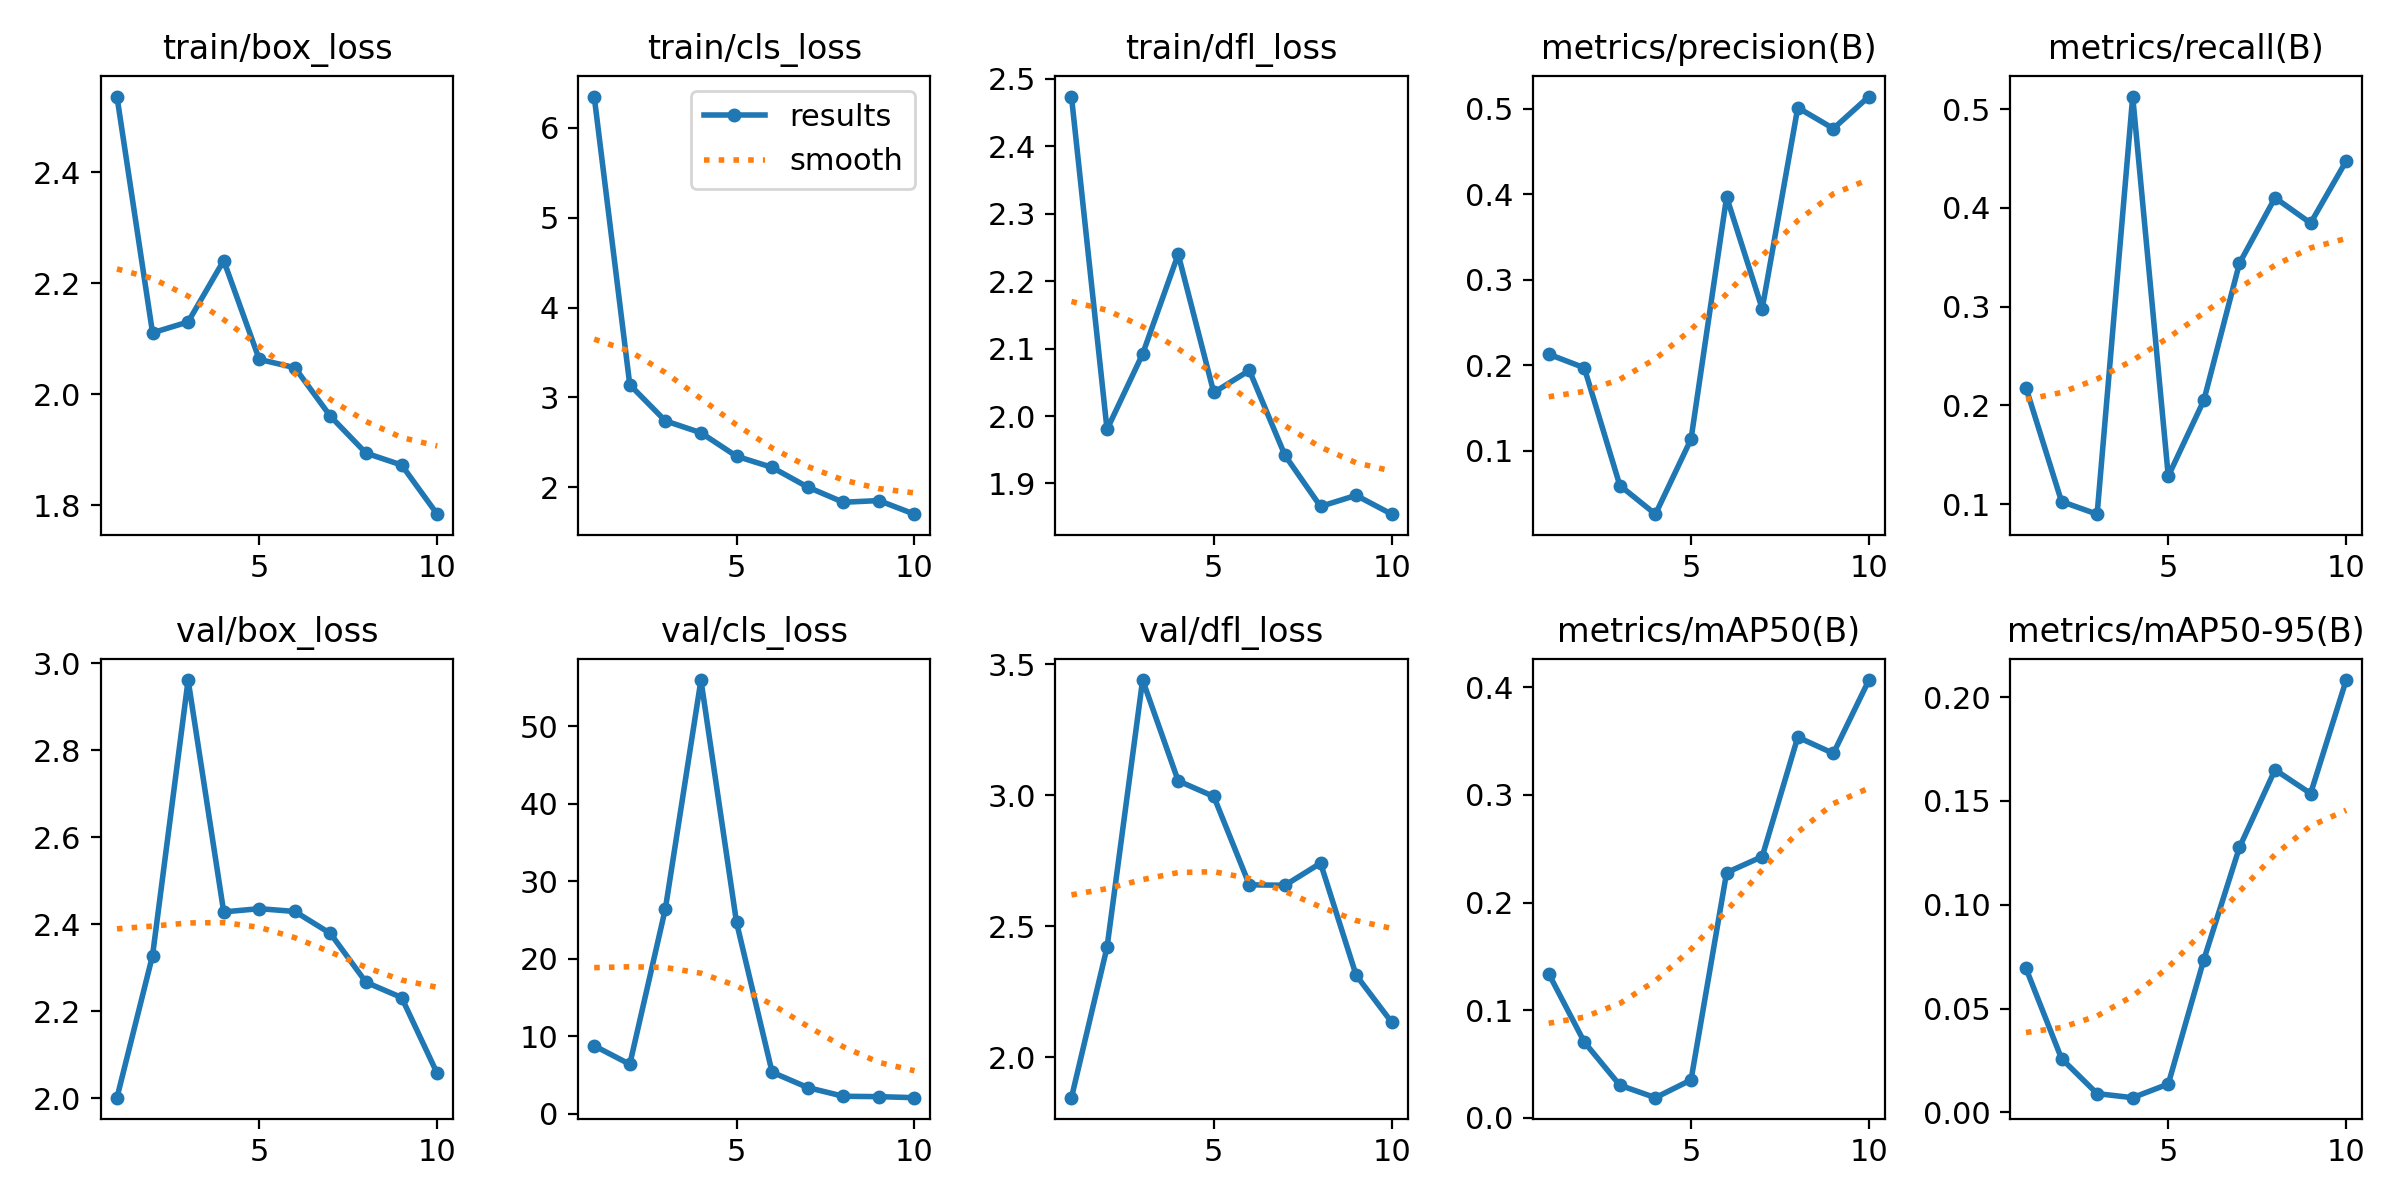
\includegraphics[width=.8\textwidth]{./figures/fig5_10e_results.png}
\caption{Model training results - 10 epochs} \label{fig5}
\end{center}
\end{figure}

Figure \ref{fig6} depicts the distribution of the F1 score, precision, and recall metrics across various confidence thresholds ranging from 0 to 1. Analyzing the F1 score curve reveals that the highest F1 score occurs at a confidence threshold of 0.275, indicating the optimal balance between precision and recall at this threshold. This observation is supported by the precision and recall curves, which show an inverse relationship: precision increases with higher confidence levels, while recall decreases.

Additionally, the data clearly indicate over fitting around a confidence threshold of 0.837, where precision reaches a perfect score of 1. Conversely, recall significantly drops at this threshold. This over fitting is likely due to the model being overly familiar with siphovirus occurrences and the lack of variability in the dataset.

\begin{figure}[H]
    
    \begin{subfigure}[b]{0.25\textwidth}
        \begin{center}
        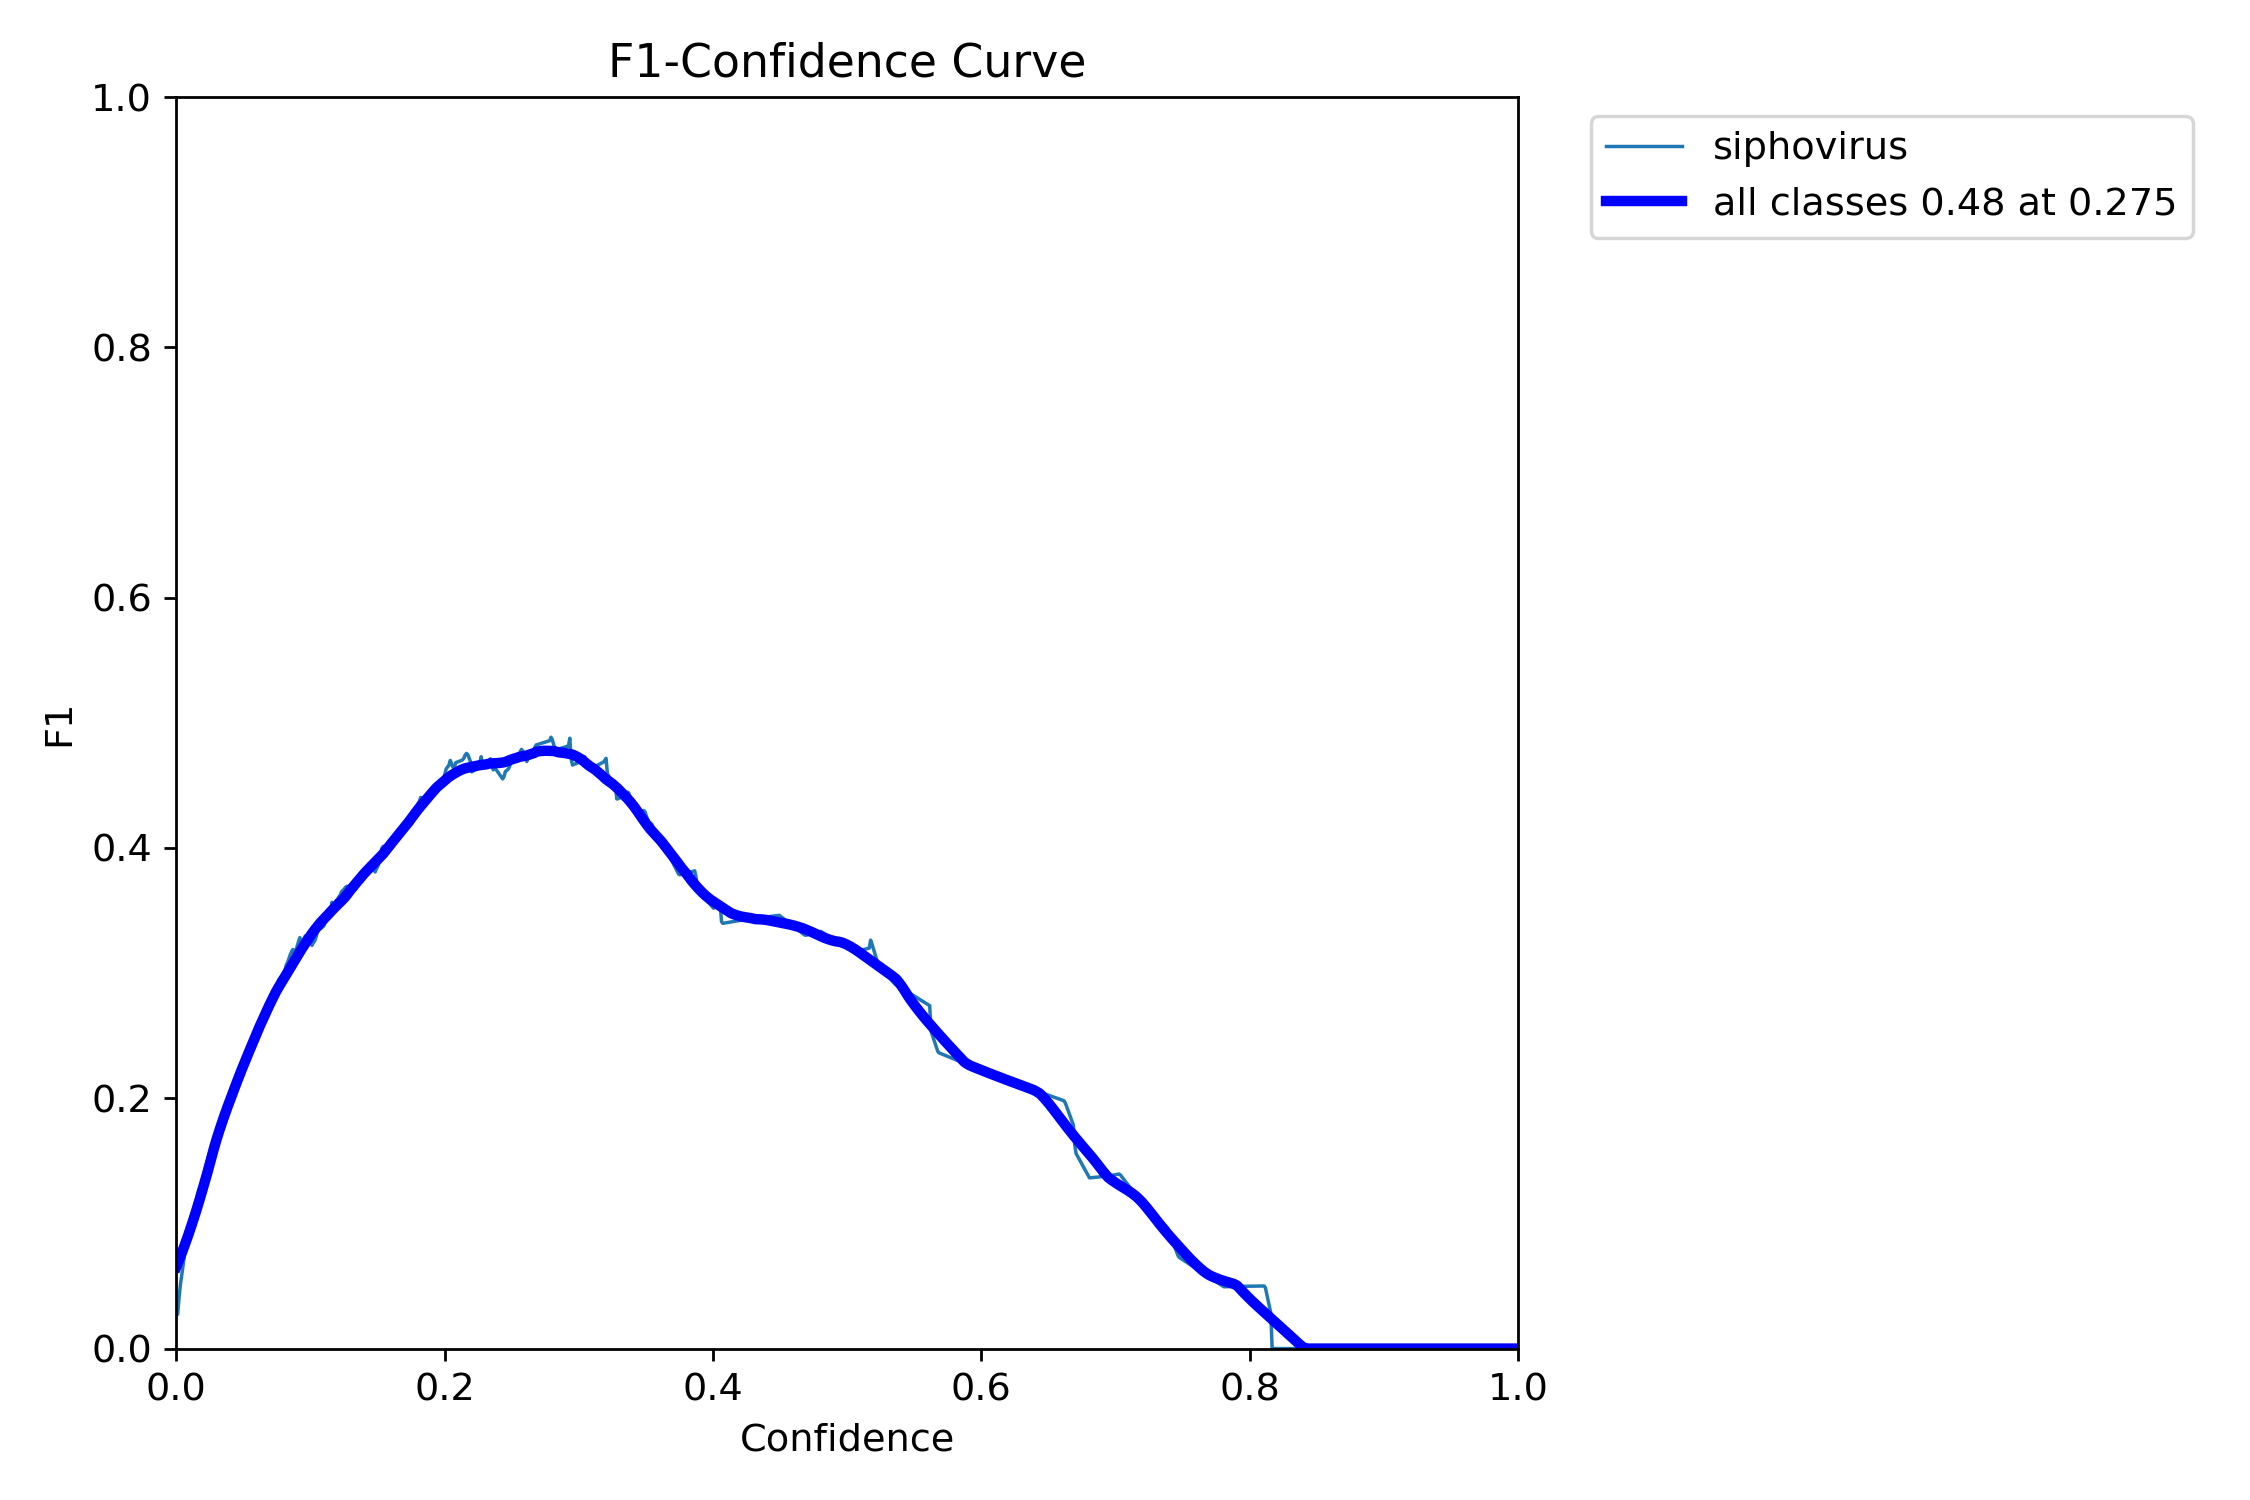
\includegraphics[height = 100px]{./figures/fig6a10e_f1_curve.png}
        \caption{F1 Score}
        \end{center}
    \end{subfigure}
    \hfill
    \begin{subfigure}[b]{0.25\textwidth}
    \begin{center}
        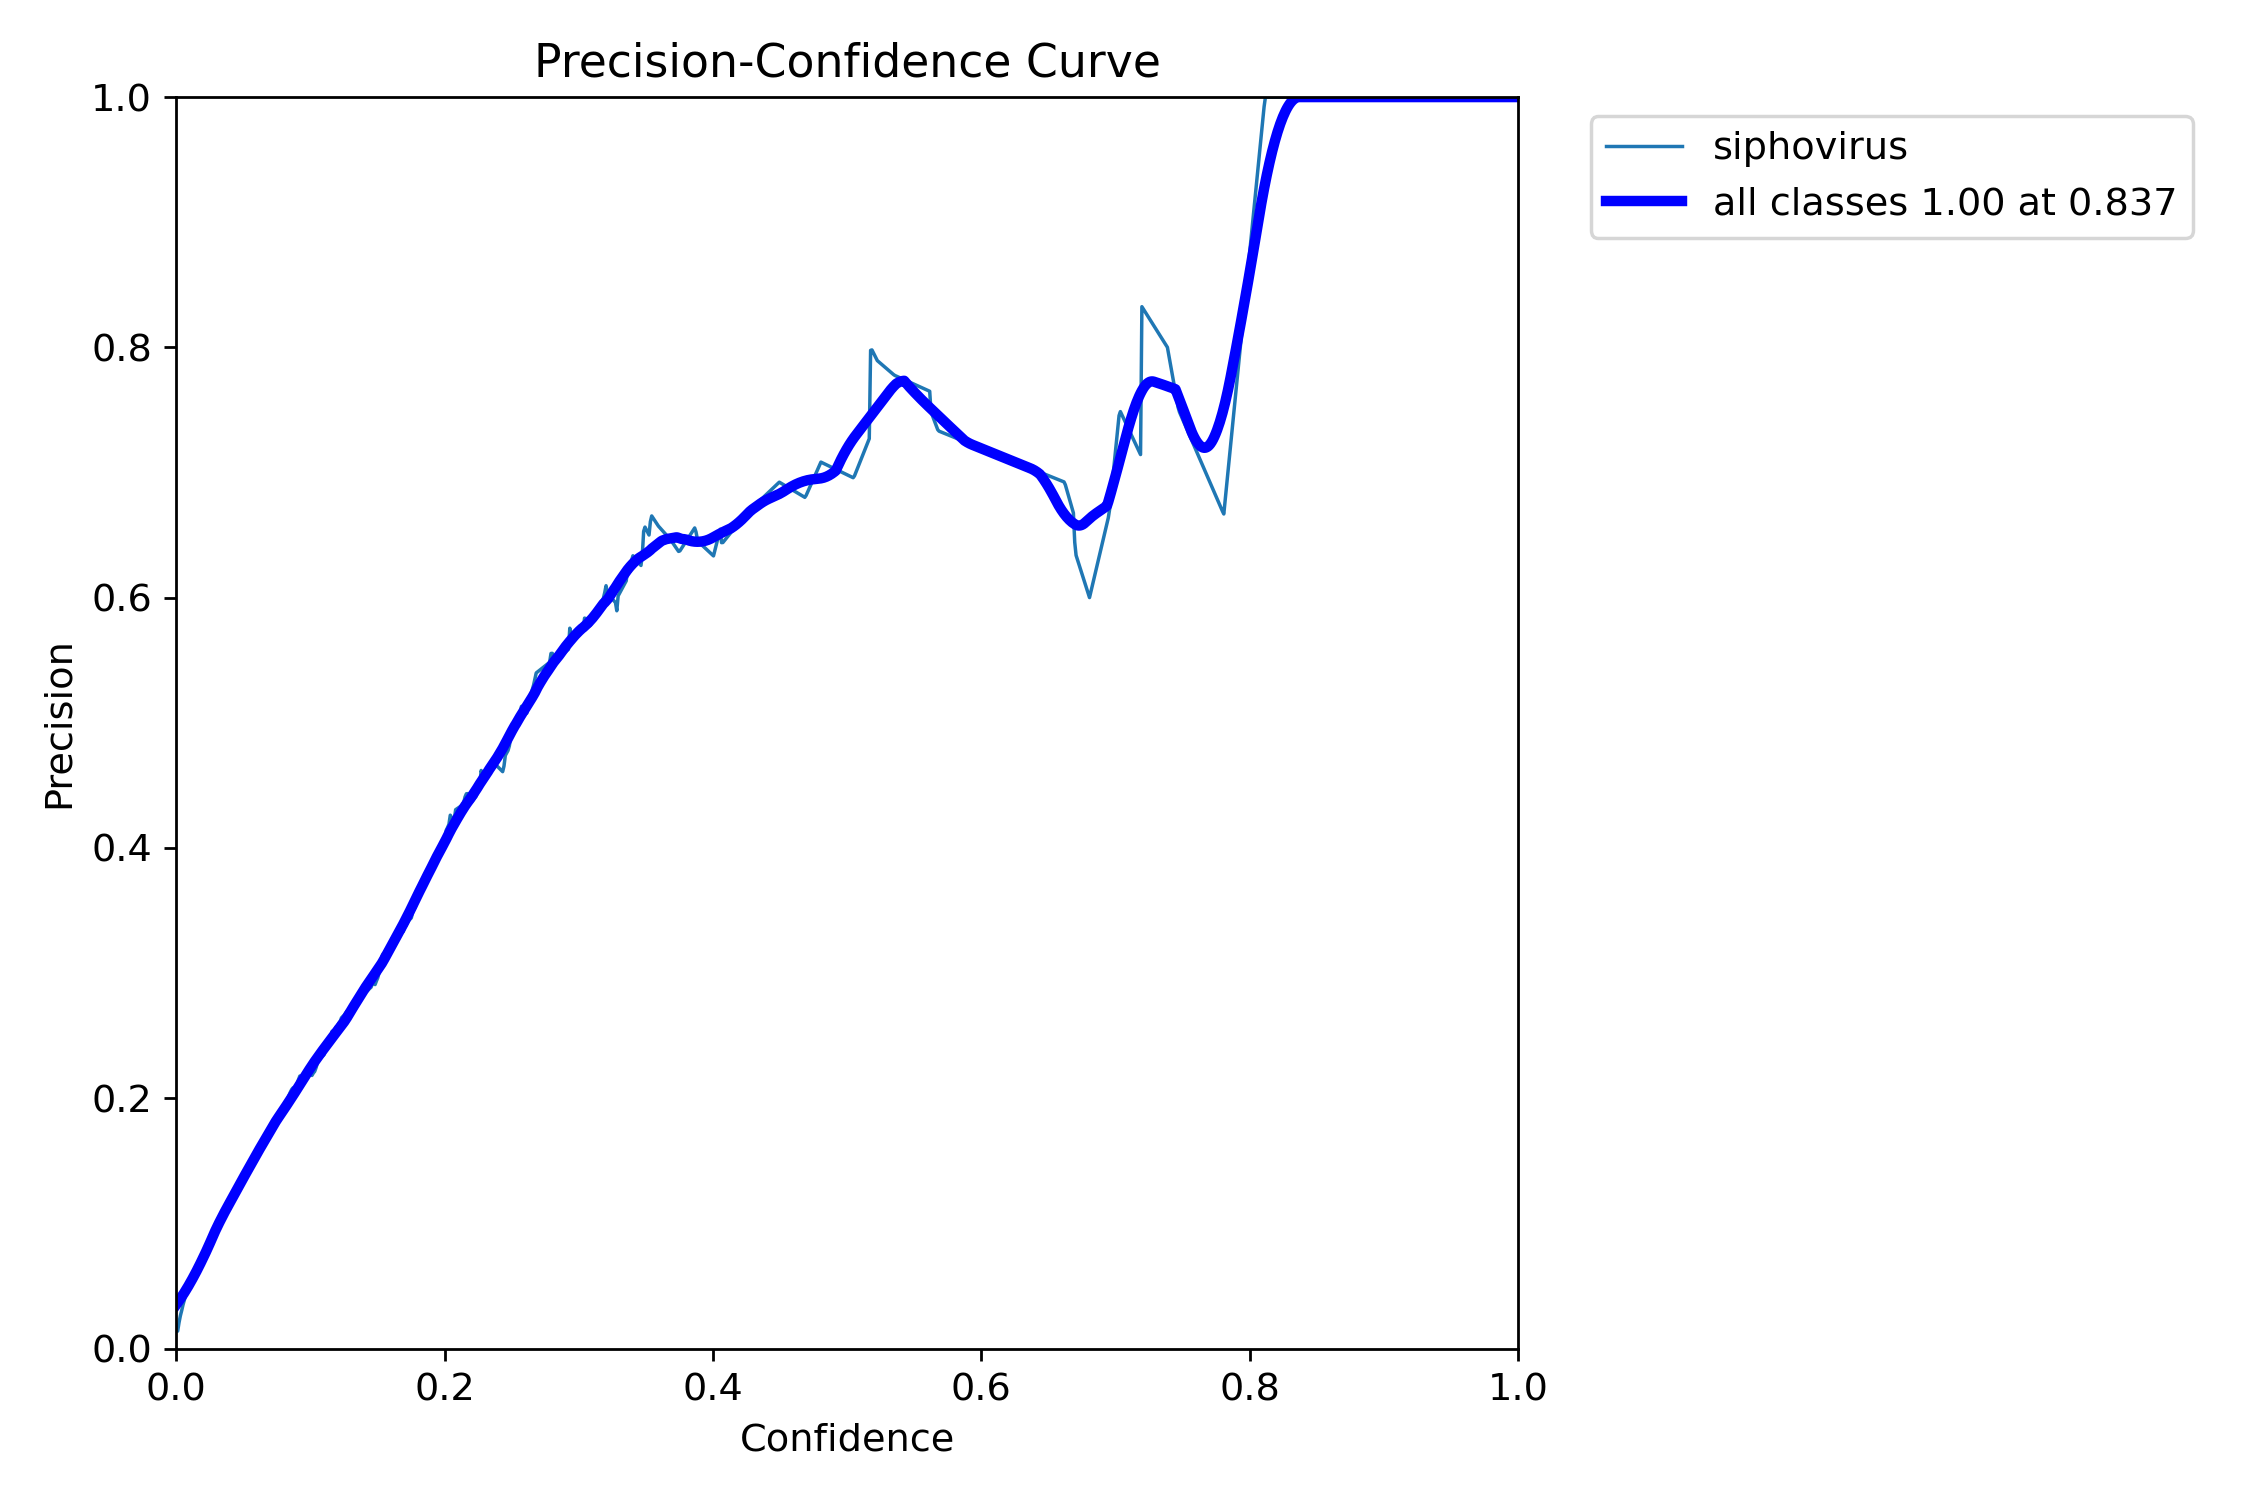
\includegraphics[height = 100px]{./figures/fig6b10e_P_curve.png}
        \caption{Precision}
        \end{center}
    \end{subfigure}
    \hfill
    \begin{subfigure}[b]{0.25\textwidth}
    \begin{center}
        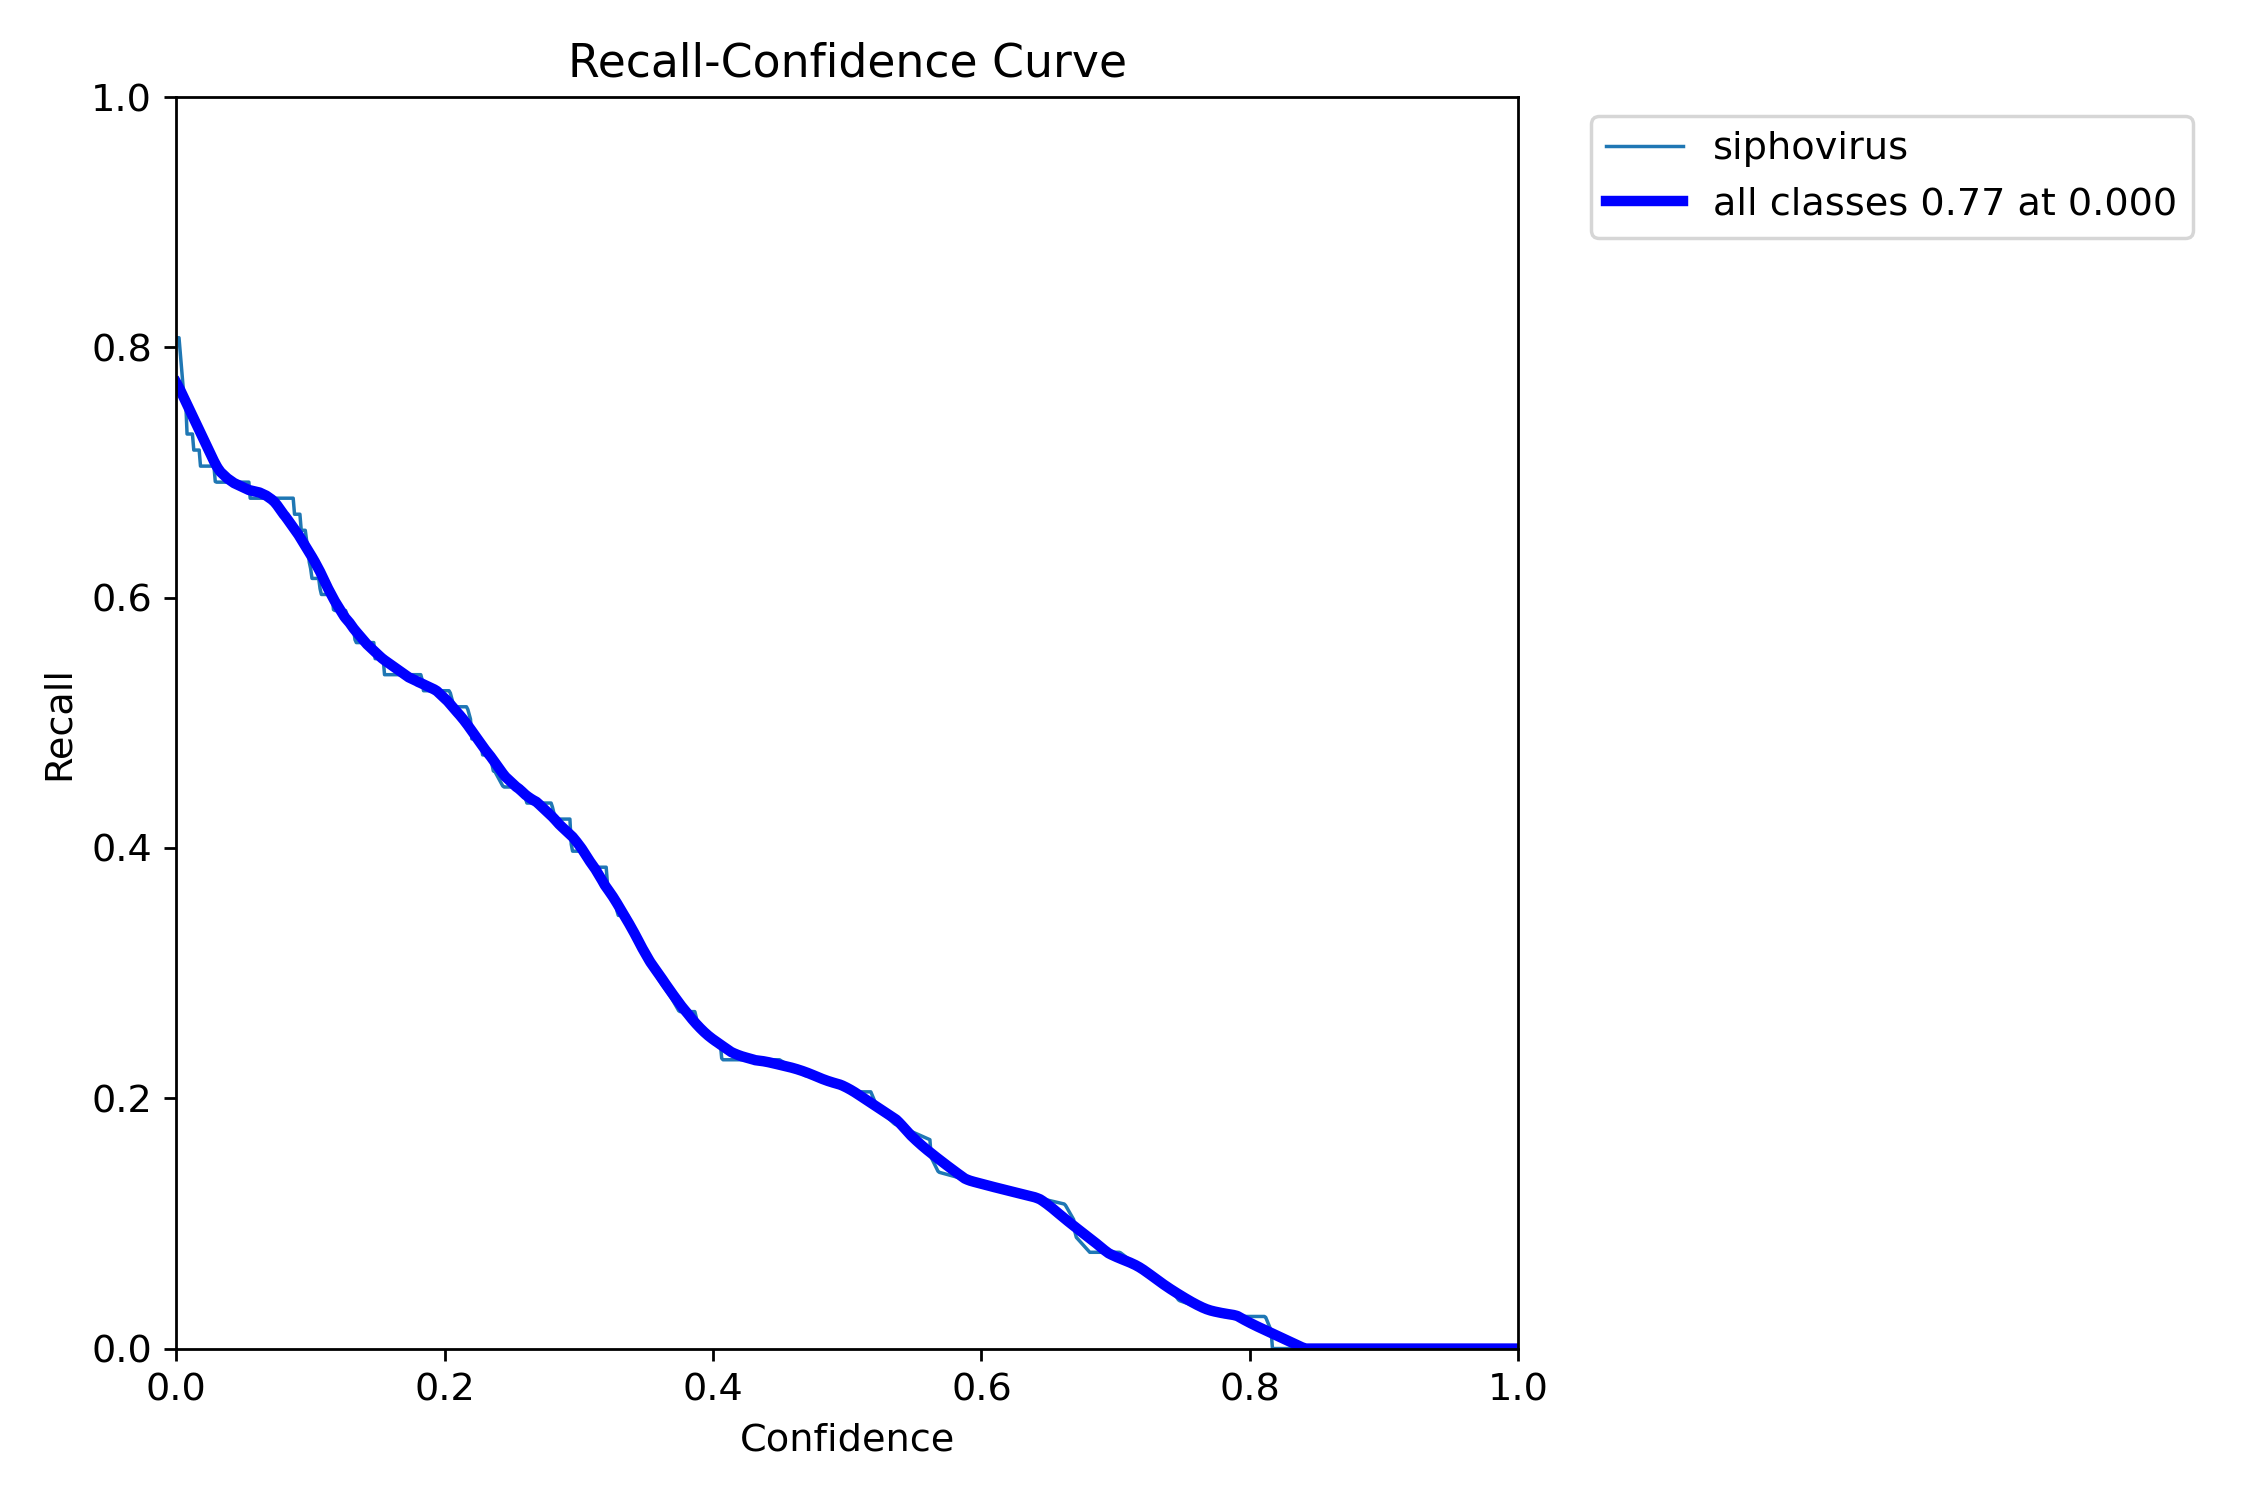
\includegraphics[height = 100px]{./figures/fig6c_10_eR_curve.png}
        \caption{Recall}
        \end{center}
    \end{subfigure}
    \caption{Performance metrics vs confidence threshold (10 epochs)}
    \label{fig6}
\end{figure}

Figure \ref{fig7} demonstrates the model's ability to infer and classify siphoviruses in micrographs. Considering the previously analyzed performance metrics and results, it is evident that the model can accurately identify and classify siphoviruses under various contrast settings (e.g., dark-stained and white-stained capsids). Although the model occasionally makes incorrect detections and partial classifications, these results indicate a solid starting point. As we will demonstrate in the following section, further training with additional epochs yields improved results.

It is noteworthy, however, that the model exhibits signs of overfitting and bias due to the extensive training on siphoviruses. Incorporating training with additional classes will likely produce different results, especially given the similarities between siphoviruses and myoviruses in their relaxed states.

\begin{figure}[H]
\begin{center}
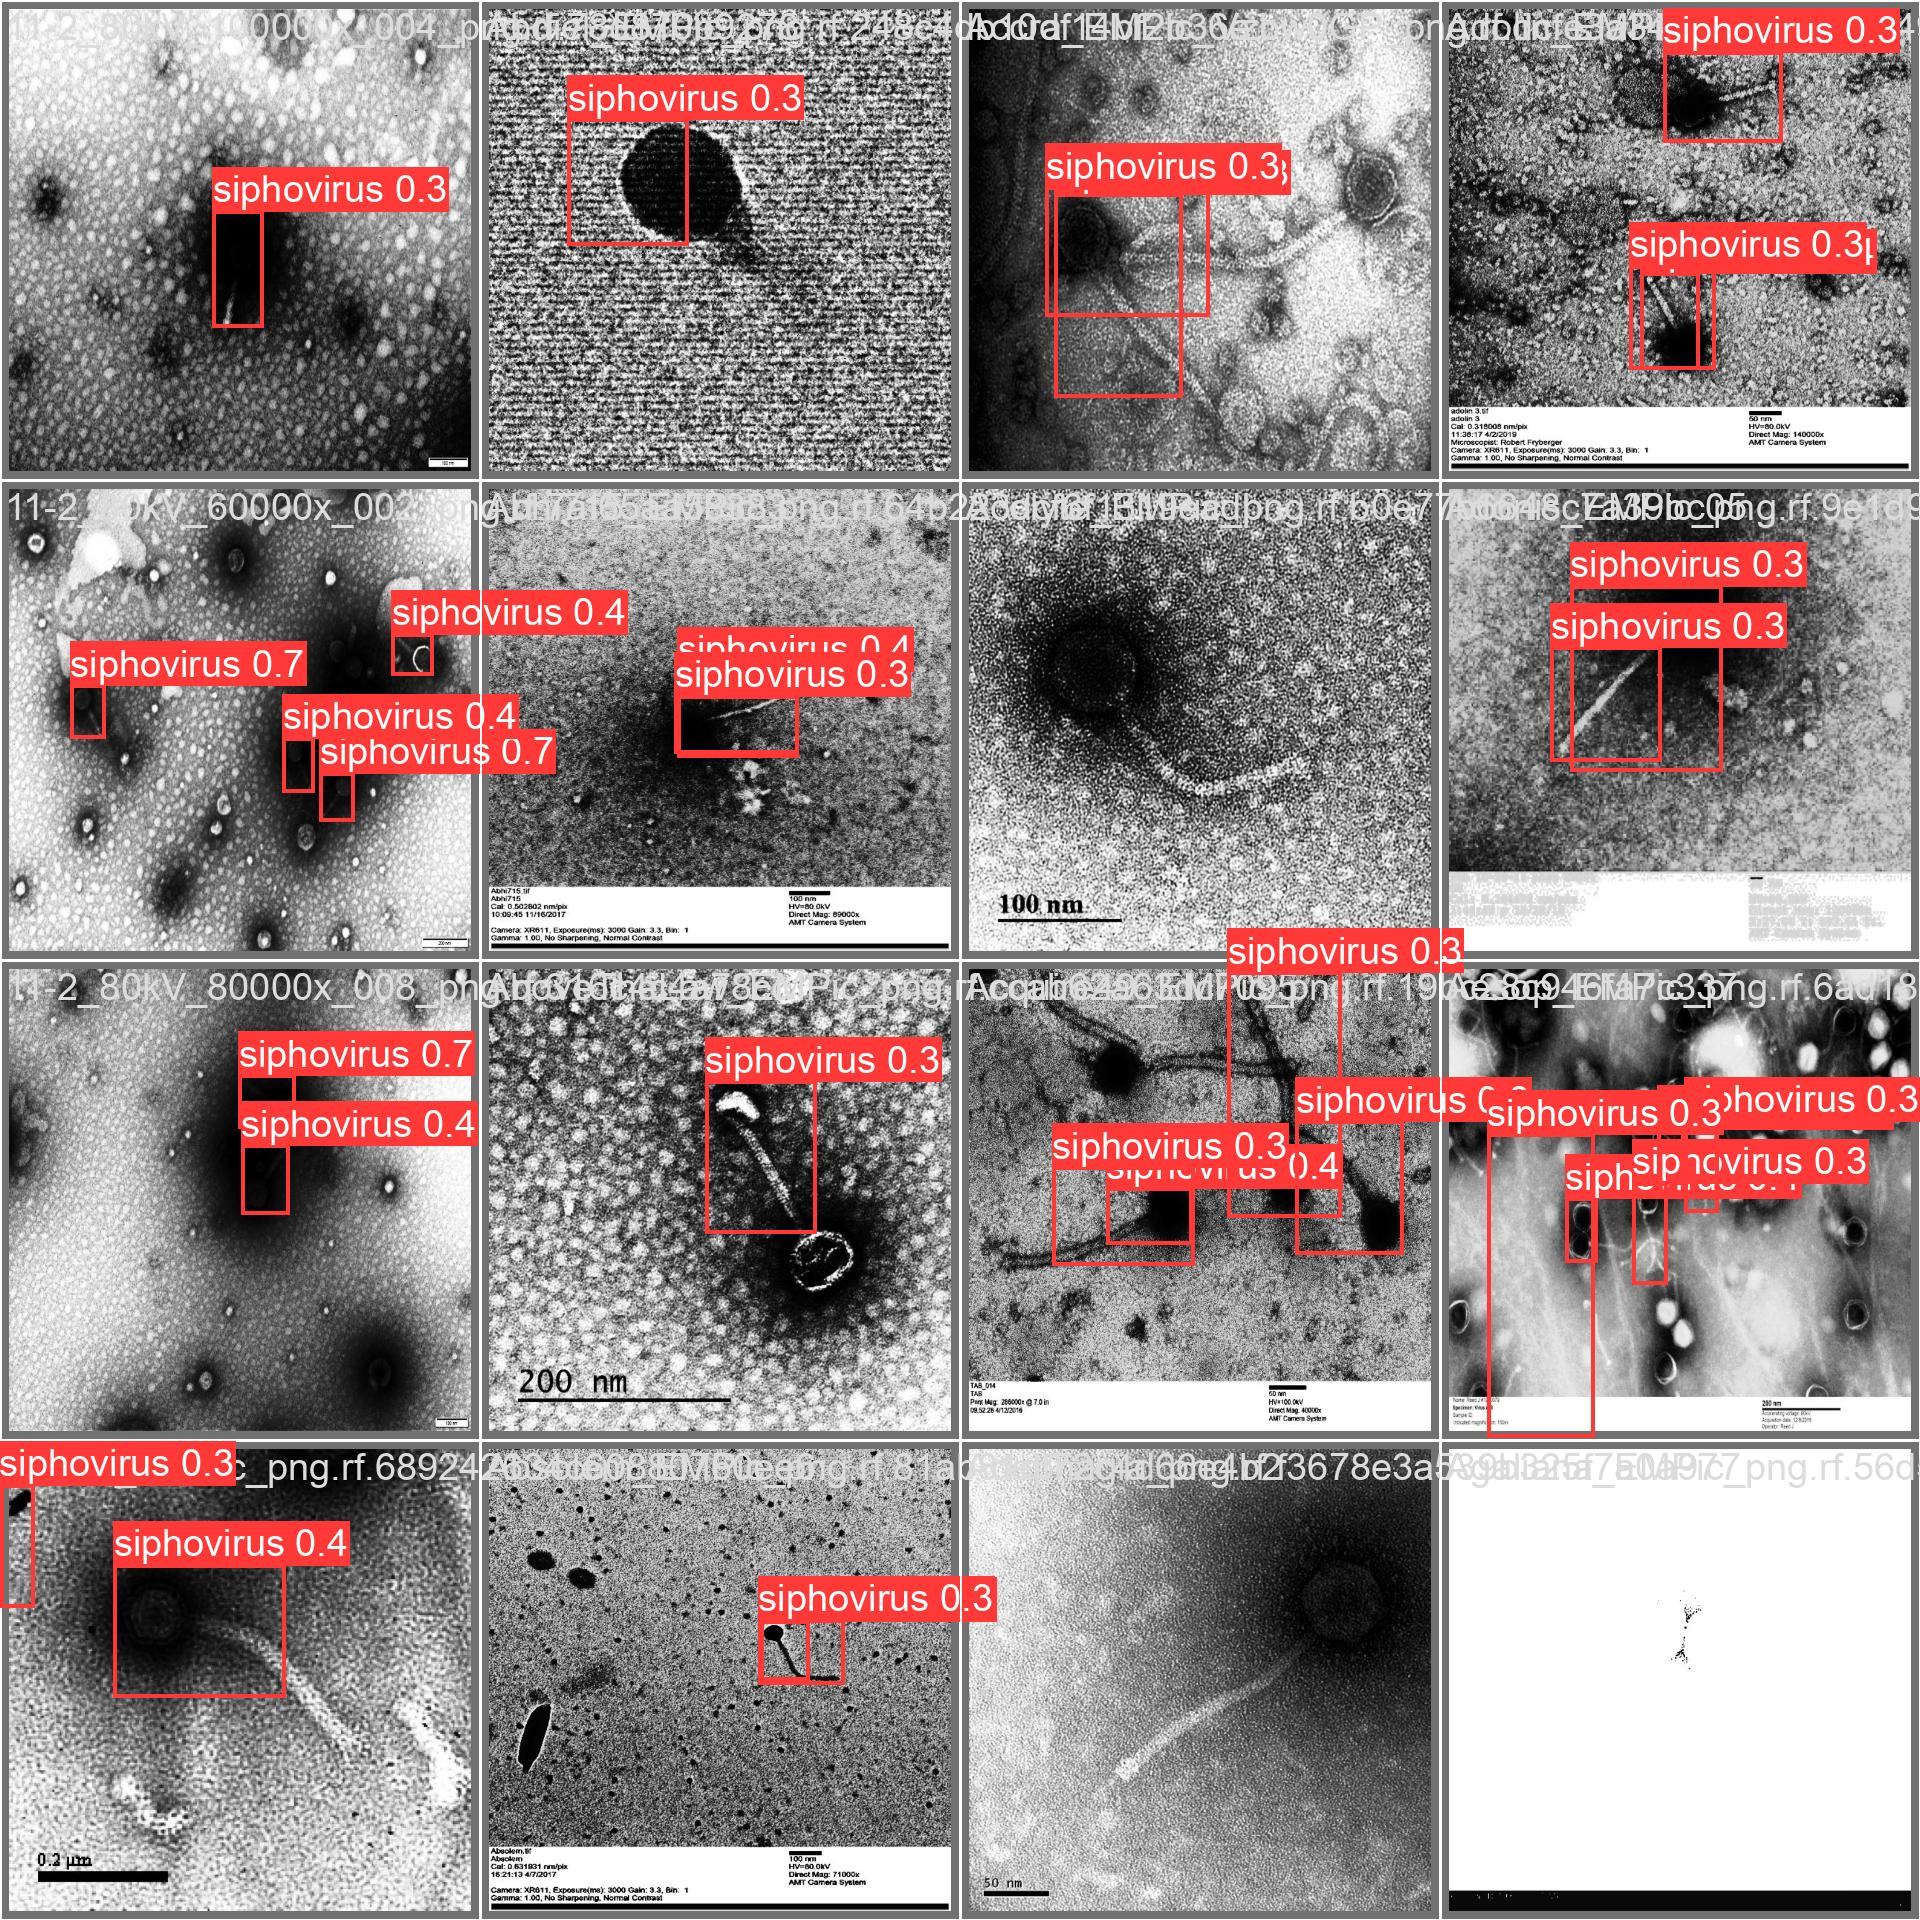
\includegraphics[width=.4\textwidth]{./figures/fig7_10e_val_batch0_pred.jpg}
\caption{Performance for validation batch - 10 epochs} \label{fig7}
\end{center}
\end{figure}

\subsection{Training results - 25 Epochs}

Figure \ref{fig8} presents the main training metrics for the model trained over 25 epochs. Similar to the previous results, there is a clear improvement in model performance with increased training epochs. Compared to the model trained for 10 epochs, all metrics show enhanced performance, including a slight reduction in box and distribution focal losses (DFL) and a significant decline in class loss. Precision, average precision, and recall have also improved.

The upward trend and the absence of plateau behavior are evident, suggesting that the model could continue to improve with further training beyond 25 epochs.

\begin{figure}[H]
\begin{center}
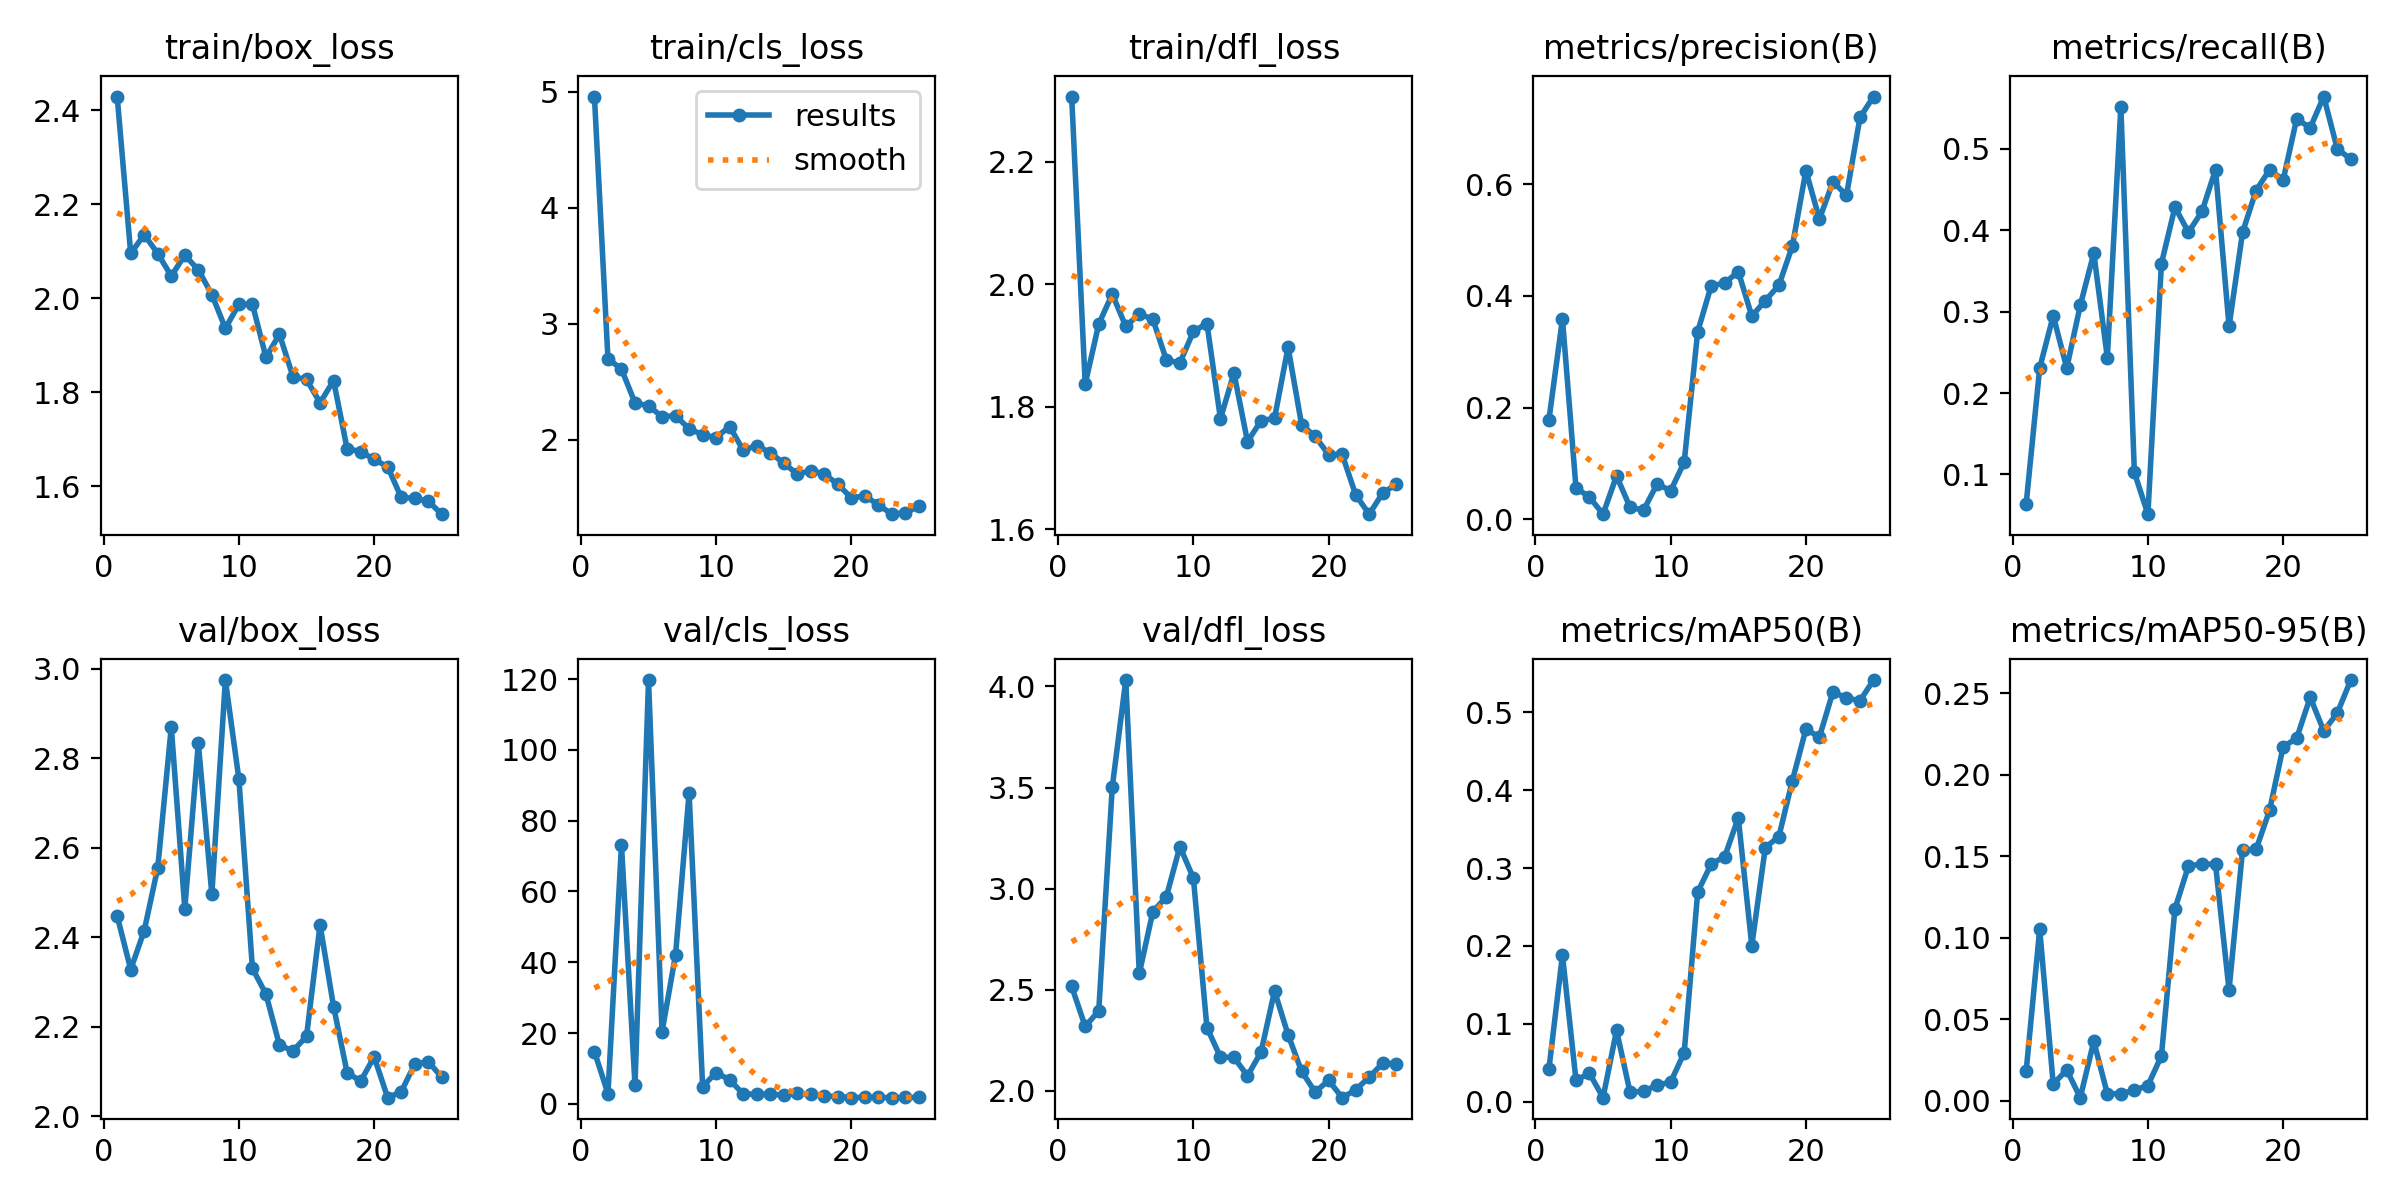
\includegraphics[width=0.8\textwidth]{./figures/fig8_25e_results.png}
\caption{Model training results - 25 epochs} \label{fig8}
\end{center}
\end{figure}


Figures \ref{fig9} depict the distribution of the F1 score, precision, and recall metrics across various confidence thresholds ranging from 0 to 1. There is a noticeable improvement in the F1 score, which peaks at 0.6 around a confidence threshold of 0.4, compared to the previous iteration's peak of 0.5 around a threshold of 0.3. This improvement is supported by the corresponding distributions of precision and recall. However, the overfitting behavior is still present and even more pronounced, further confirming our concerns.

\begin{figure}[H]
    
    \begin{subfigure}[b]{0.25\textwidth}
        \begin{center}
        \includegraphics[height = 100px]{./figures/fig9a_25e_f1_curve.png}
        \caption{F1 Score}
        \end{center}
    \end{subfigure}
    \hfill
    \begin{subfigure}[b]{0.25\textwidth}
    \begin{center}
        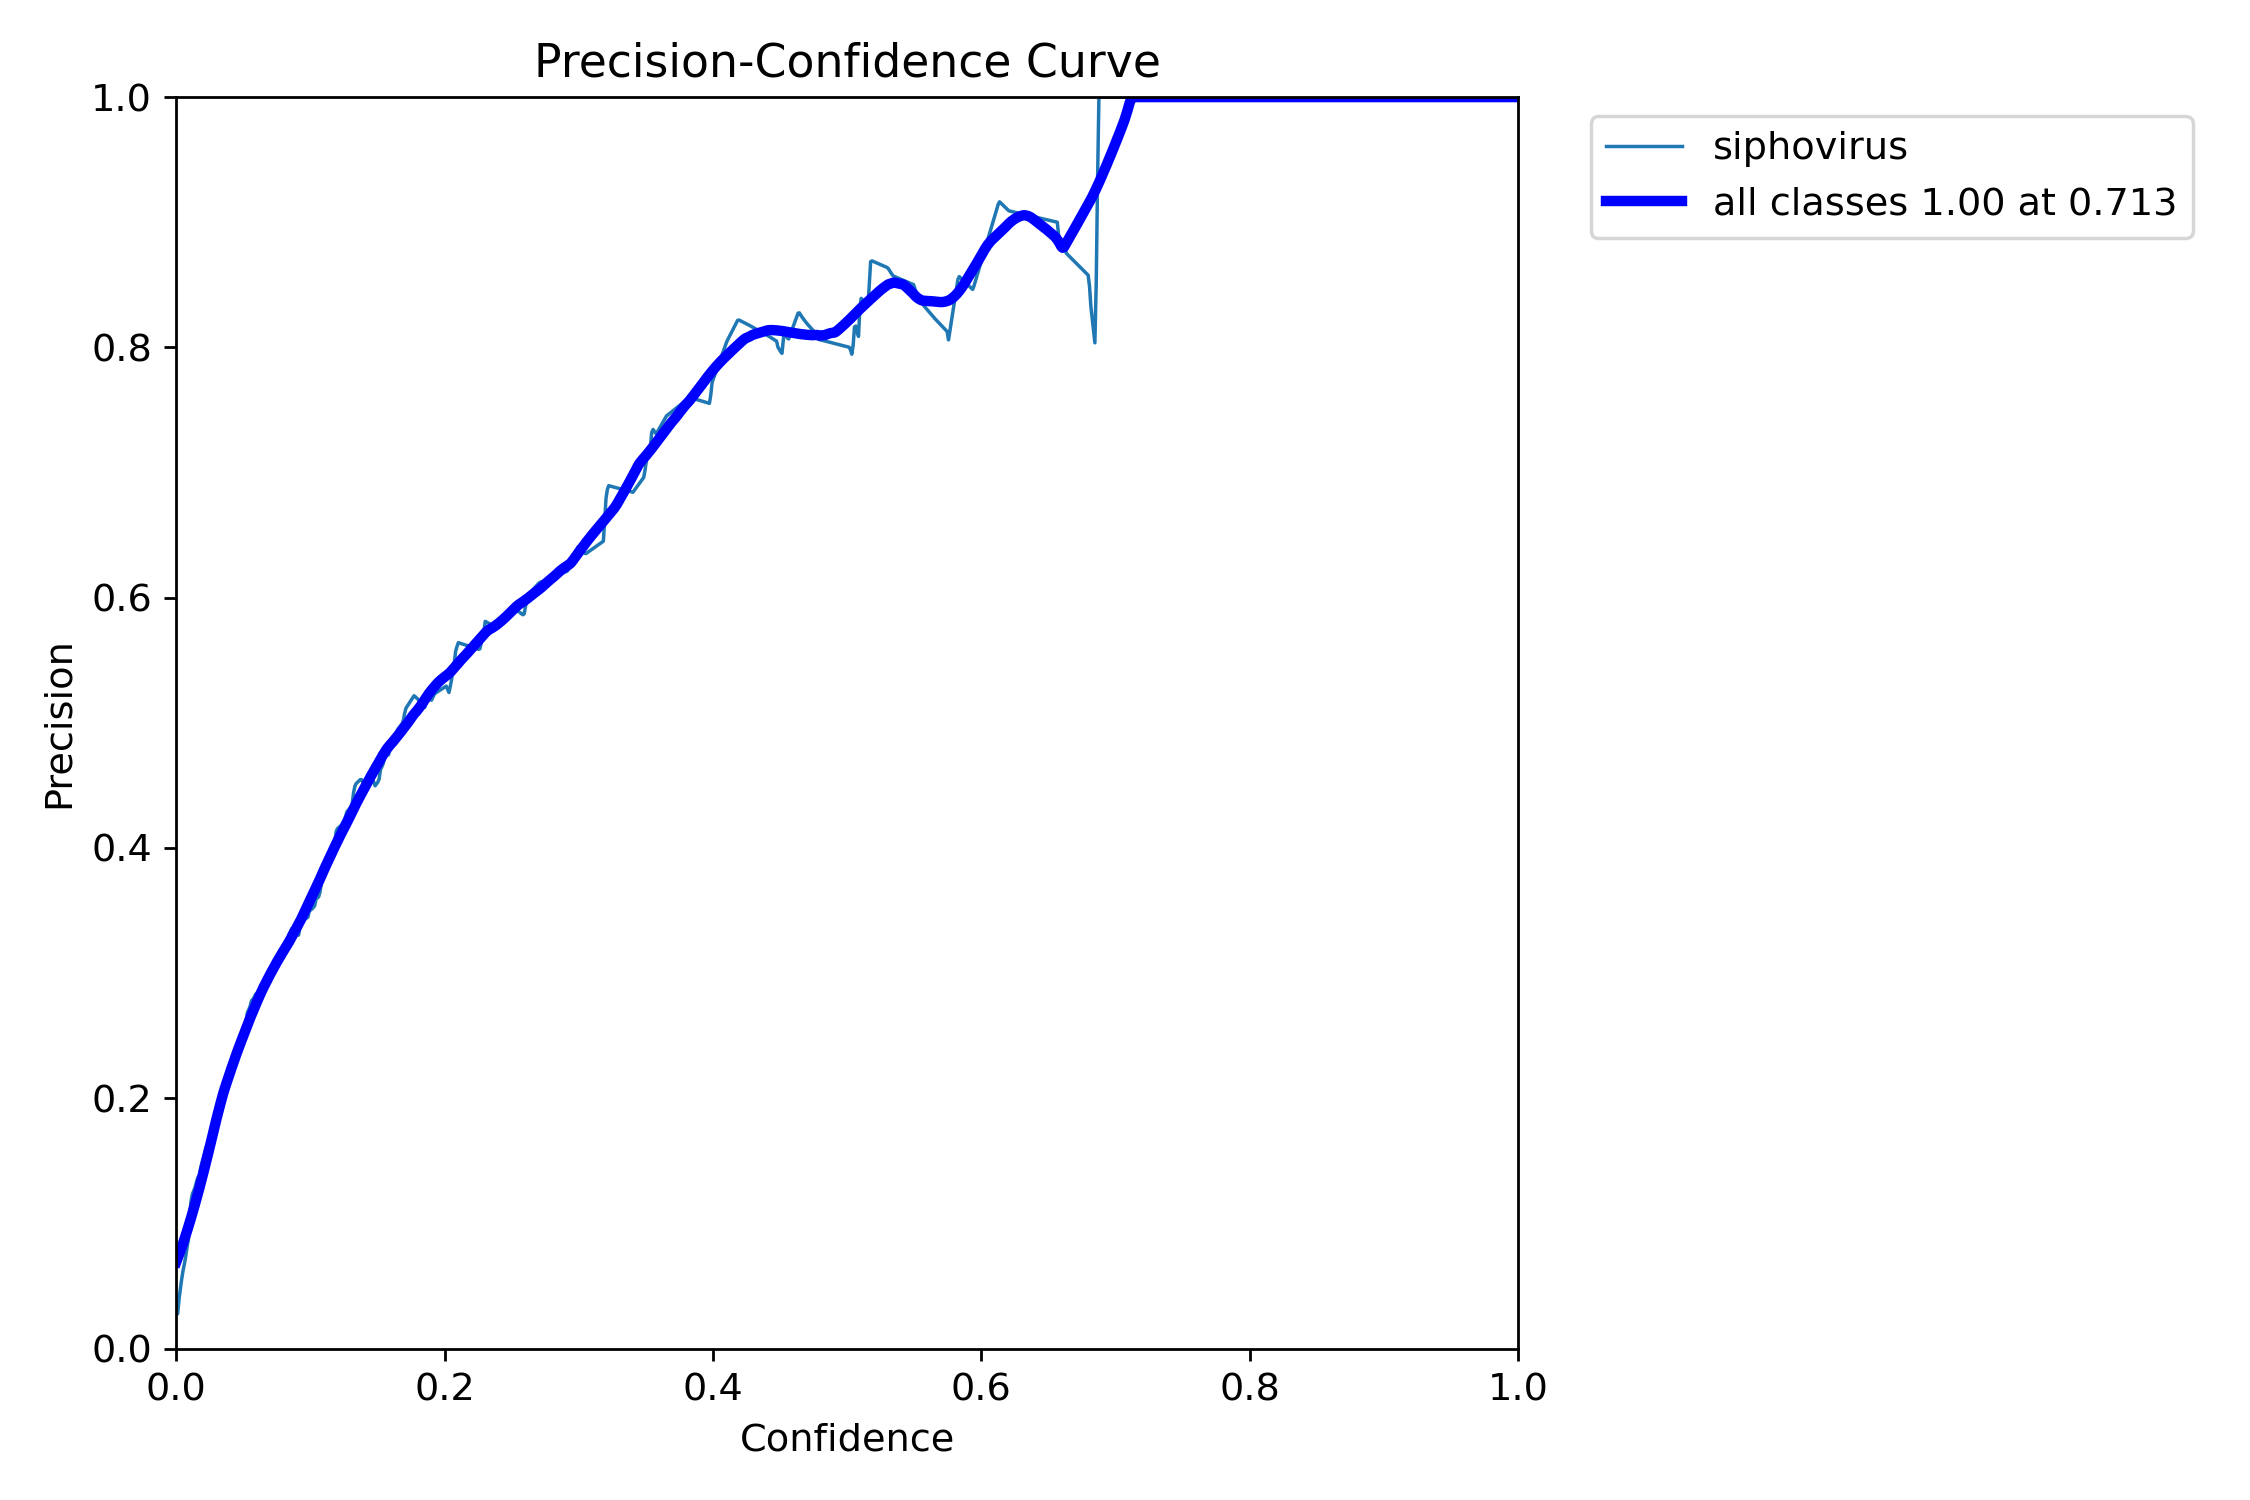
\includegraphics[height = 100px]{./figures/fig9b_25e_P_curve.png}
        \caption{Precision}
        \end{center}
    \end{subfigure}
    \hfill
    \begin{subfigure}[b]{0.25\textwidth}
    \begin{center}
        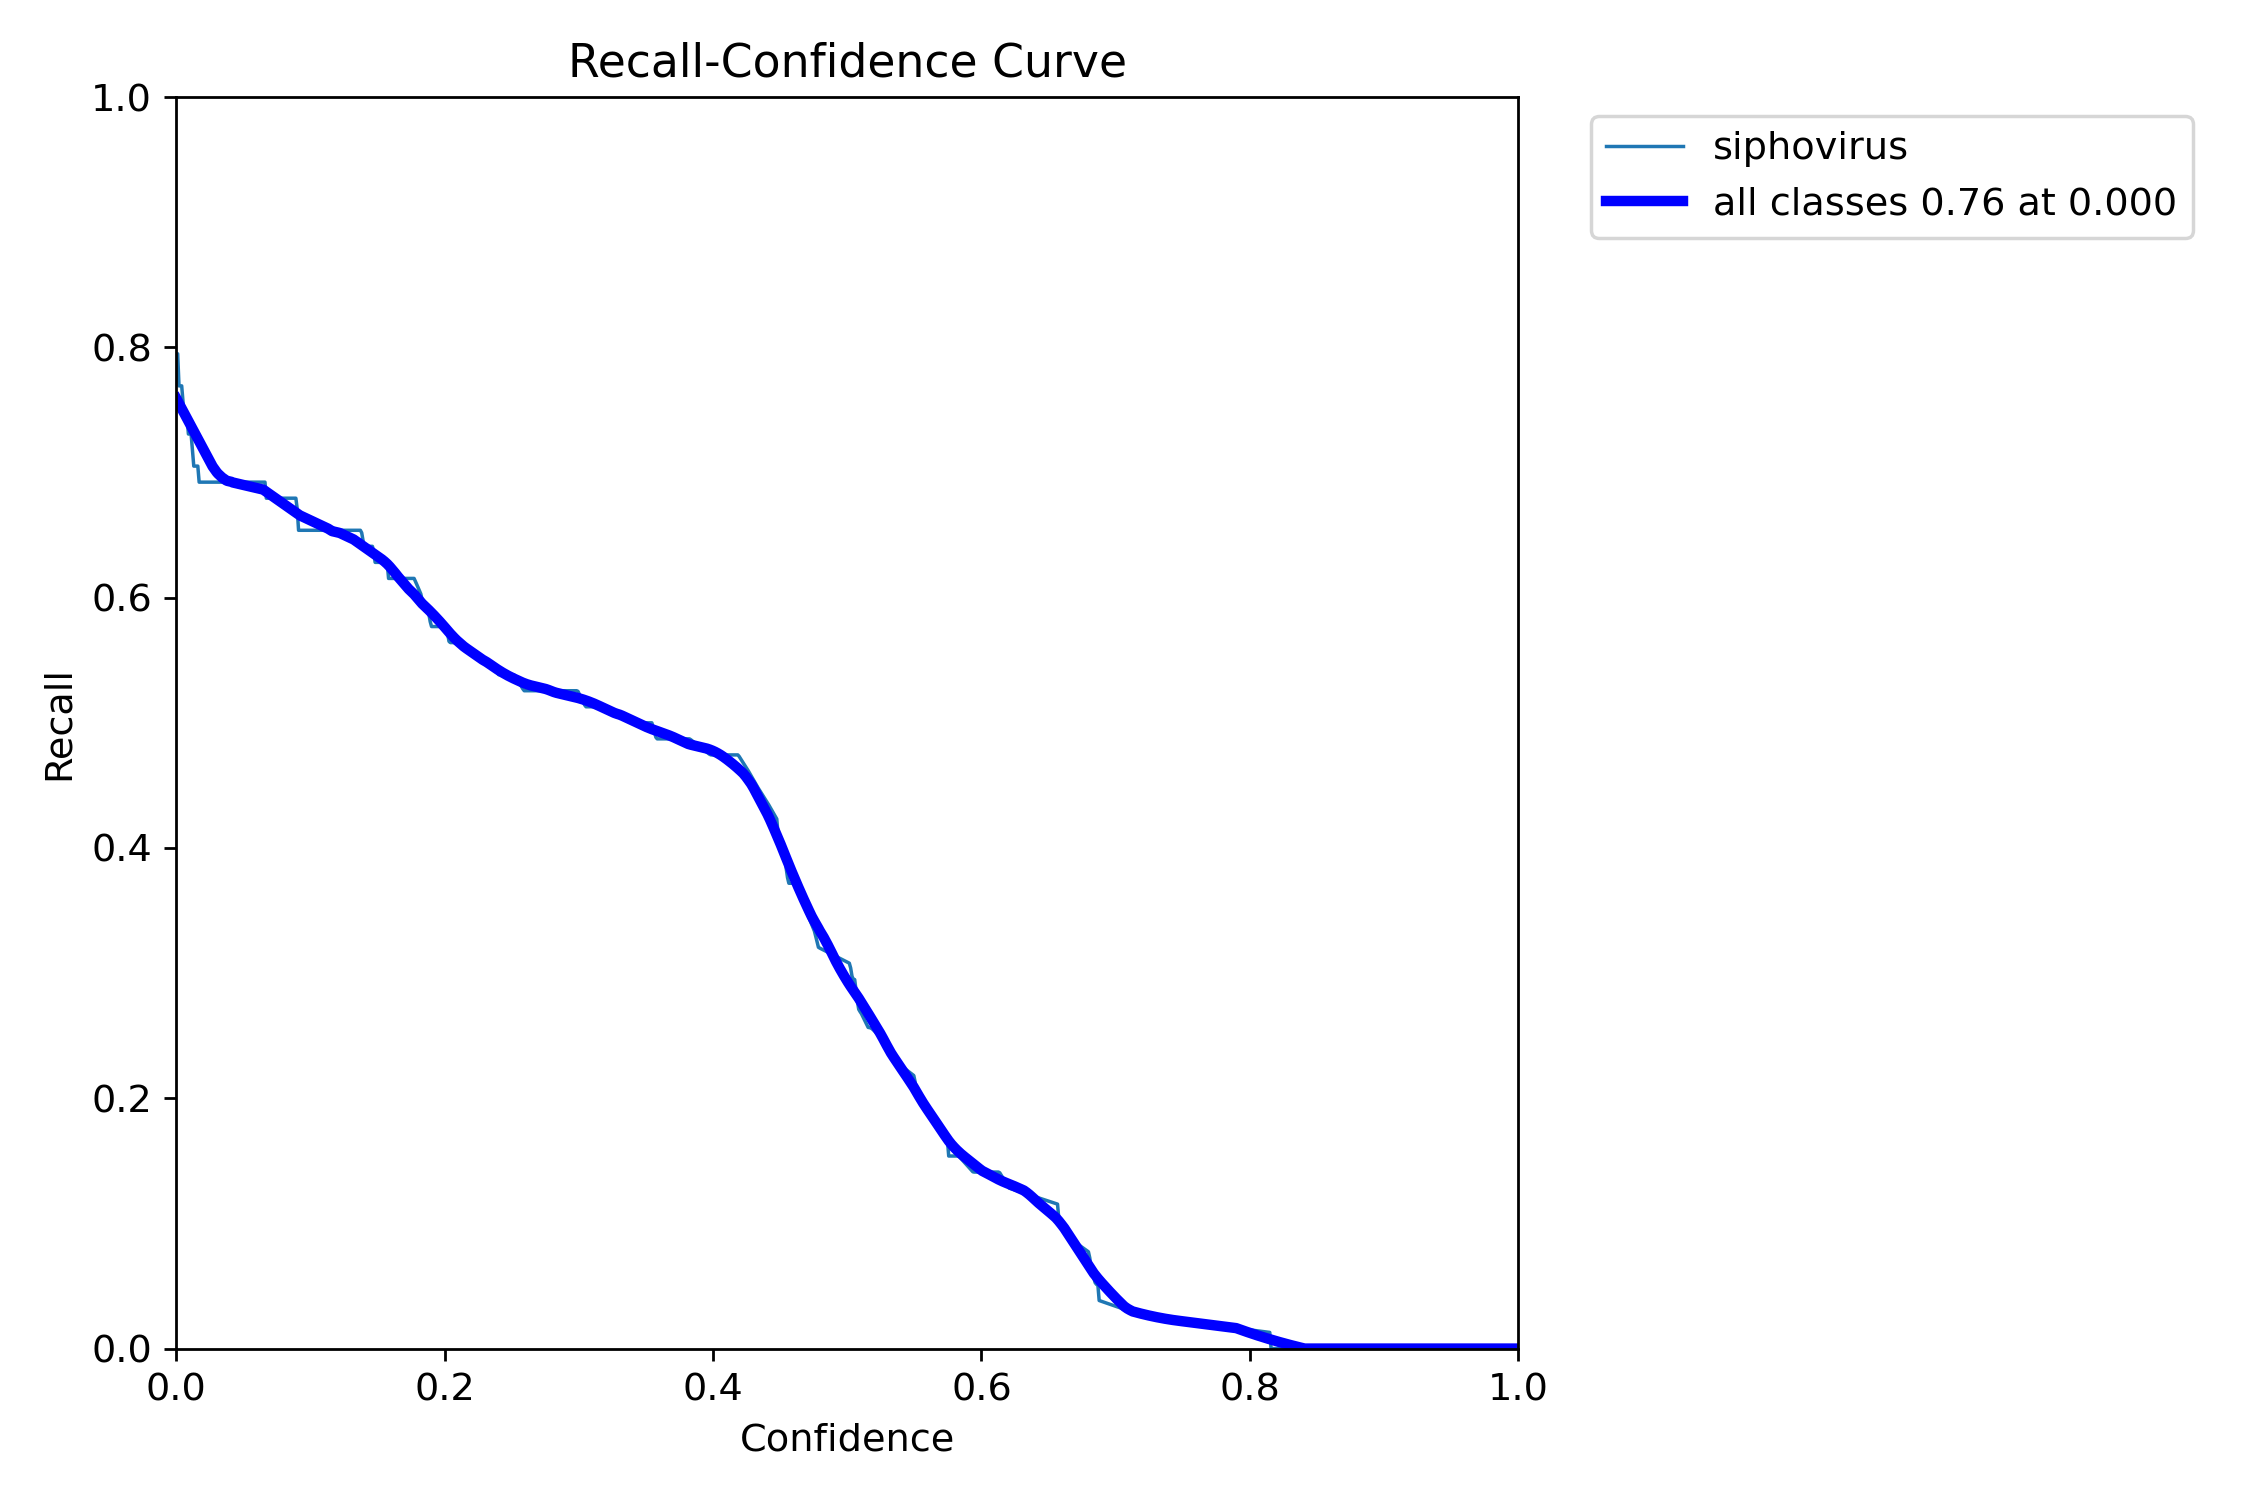
\includegraphics[height = 100px]{./figures/fig9c_25e_R_curve.png}
        \caption{Recall}
        \end{center}
    \end{subfigure}
    \caption{Performance metrics vs confidence threshold (25 epochs)}
    \label{fig9}
\end{figure}

Figure \ref{fig10} demonstrates these improvements, showing more accurate classifications and higher confidence levels for correct identifications. Despite these advancements, it is crucial to remain aware of the persistent overfitting and biases, which are likely due to the extensive number of siphovirus micrographs used during training.

\begin{figure}
\begin{center}
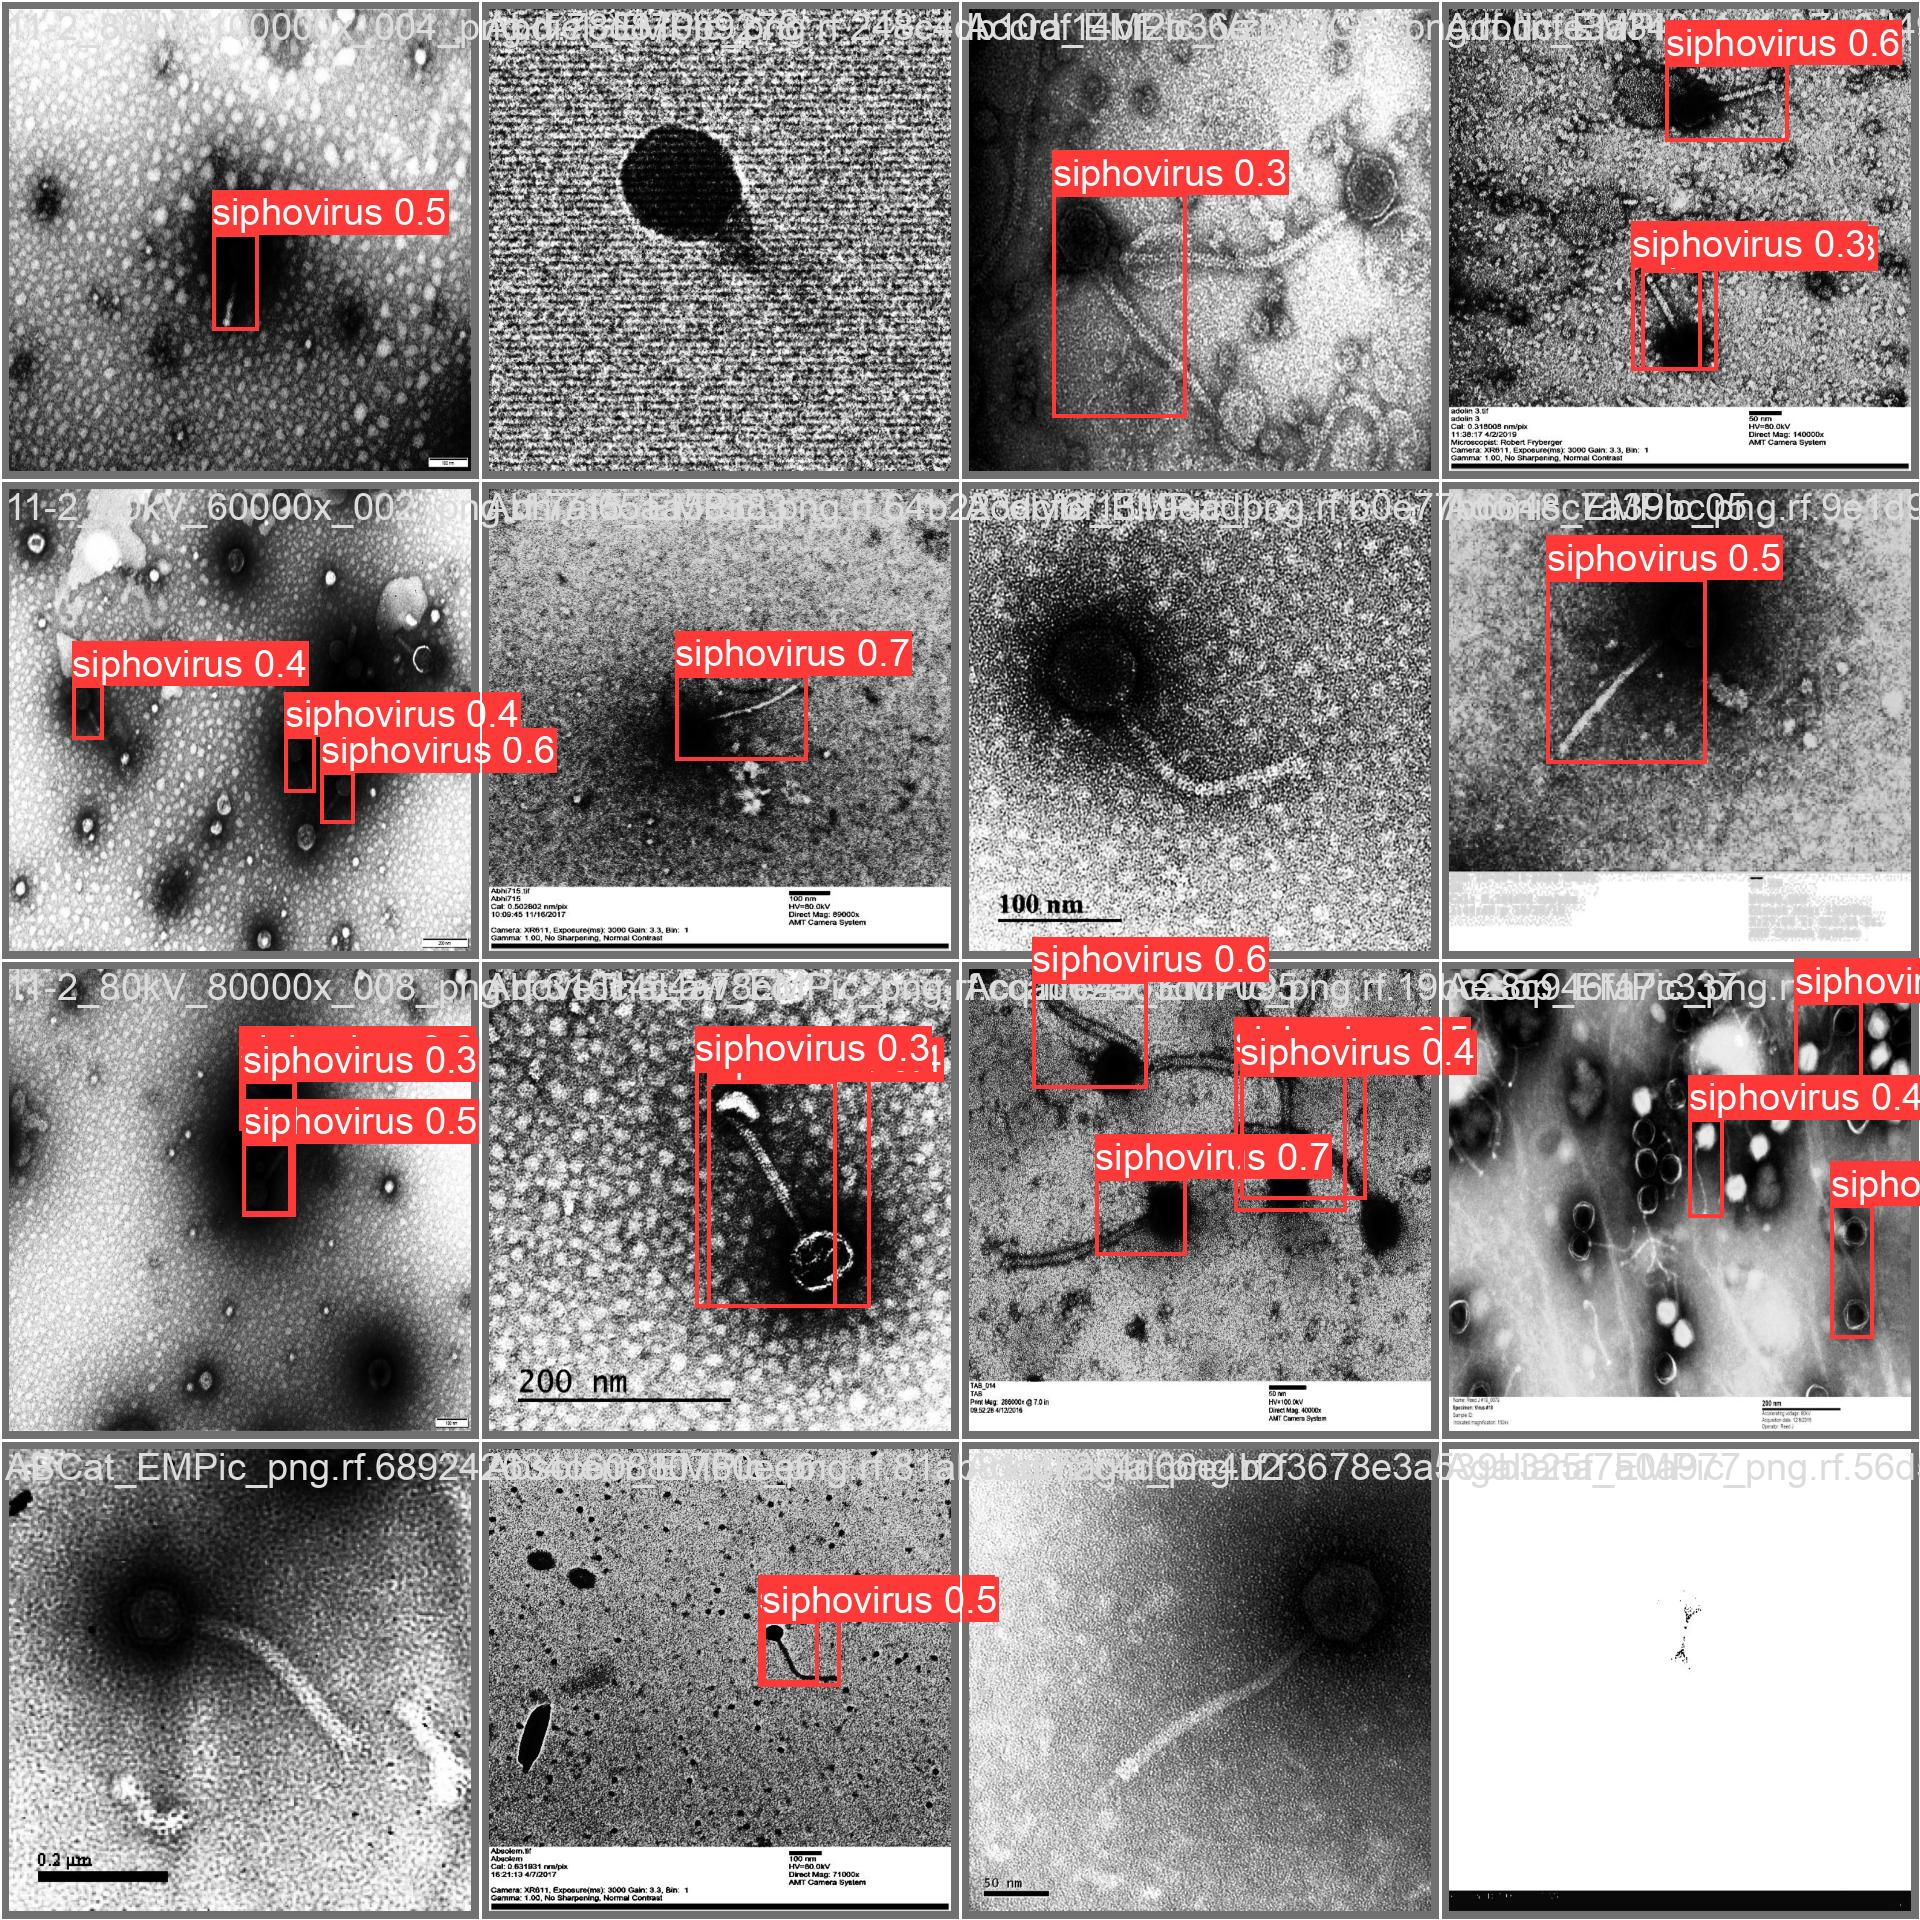
\includegraphics[width=.4\textwidth]{./figures/fig10_25e_val_batch0_pred.jpg}
\caption{Performance for validation batch - 25 epochs} \label{fig10}
\end{center}
\end{figure}

\subsection{Training results - 50 Epochs}

When the model is trained for 50 epochs, Figure \ref{fig11} shows a further improvement in box, class, and distribution focal losses (DFL). Precision and recall also improve, reaching 0.8 and 0.6, respectively. However, signs of overtraining become apparent after around 40 epochs, with precision beginning to decline. This indicates overfitting, where continued training beyond 40 epochs deteriorates performance. Implementing early stopping strategies could have addressed this issue by halting the training process when no further improvements are detected.

\begin{figure}[H]
\begin{center}
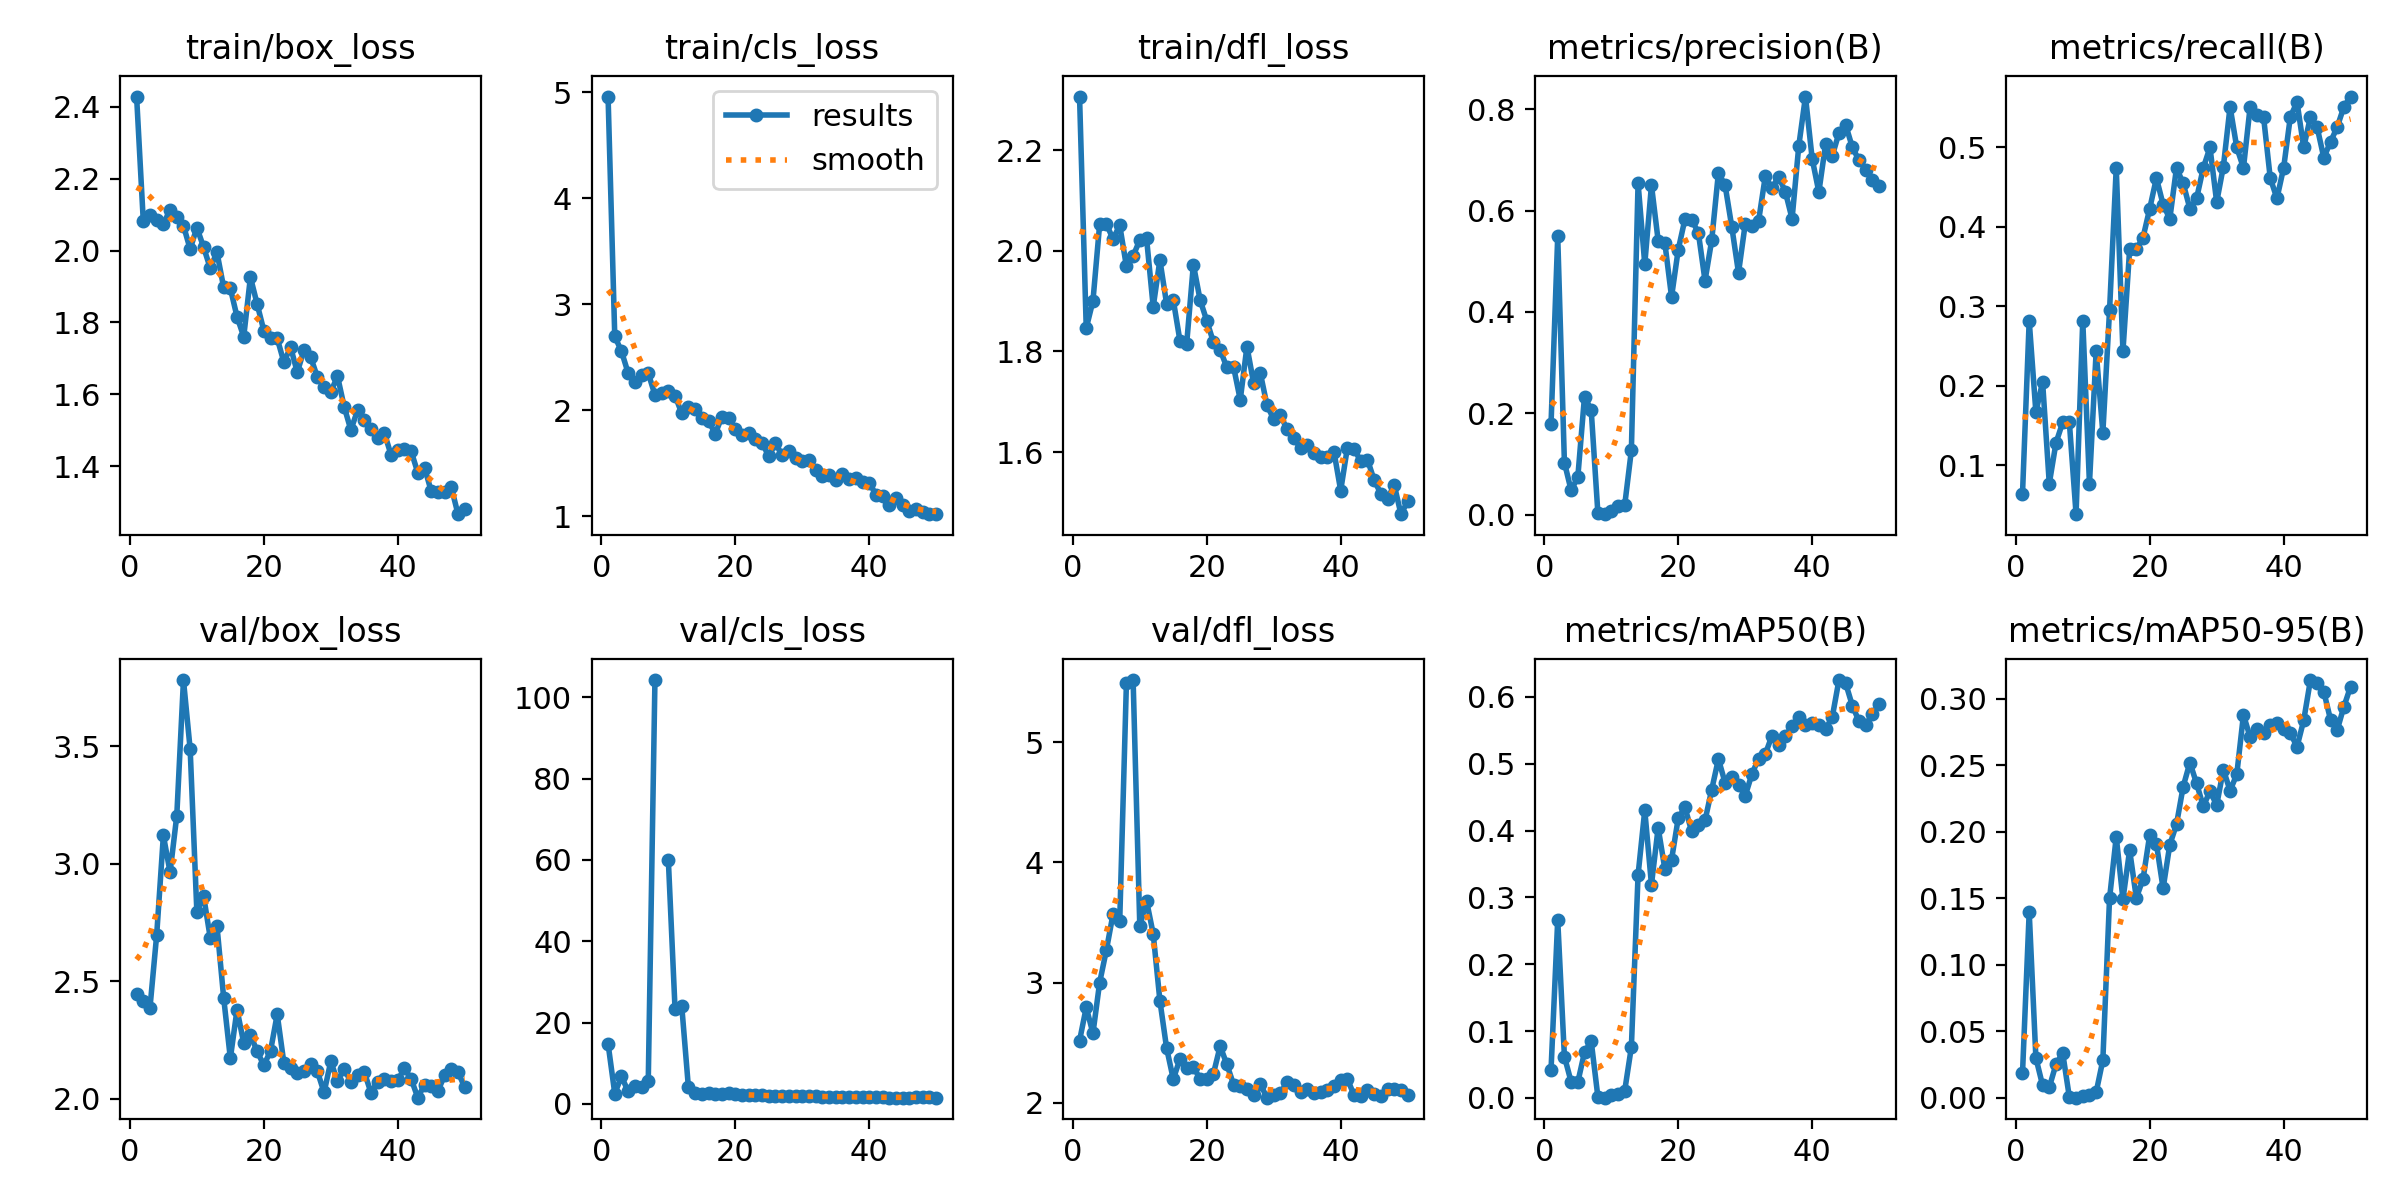
\includegraphics[width=0.8\textwidth]{./figures/fig11_50e_results.png}
\caption{Model training results - 50 epochs} \label{fig11}
\end{center}
\end{figure}

Regarding the F1 score, precision, and recall (Figure \ref{fig12}), the highest F1 score remains close to that achieved with 25 epochs, but its decline is less steep and it remains at peak level across a broader confidence threshold range. However, it is important to note that overfitting manifests much sooner, as evidenced by precision reaching a value of 1 around a 0.5 confidence threshold. Nonetheless, recall is more consistent and hits a value of 0 later, indicating improvements in this metric.

\begin{figure}[H]
    
    \begin{subfigure}[b]{0.25\textwidth}
        \begin{center}
        \includegraphics[height = 100px]{./figures/fig12a_50e_f1_curve.png}
        \caption{F1 Score}
        \end{center}
    \end{subfigure}
    \hfill
    \begin{subfigure}[b]{0.25\textwidth}
    \begin{center}
        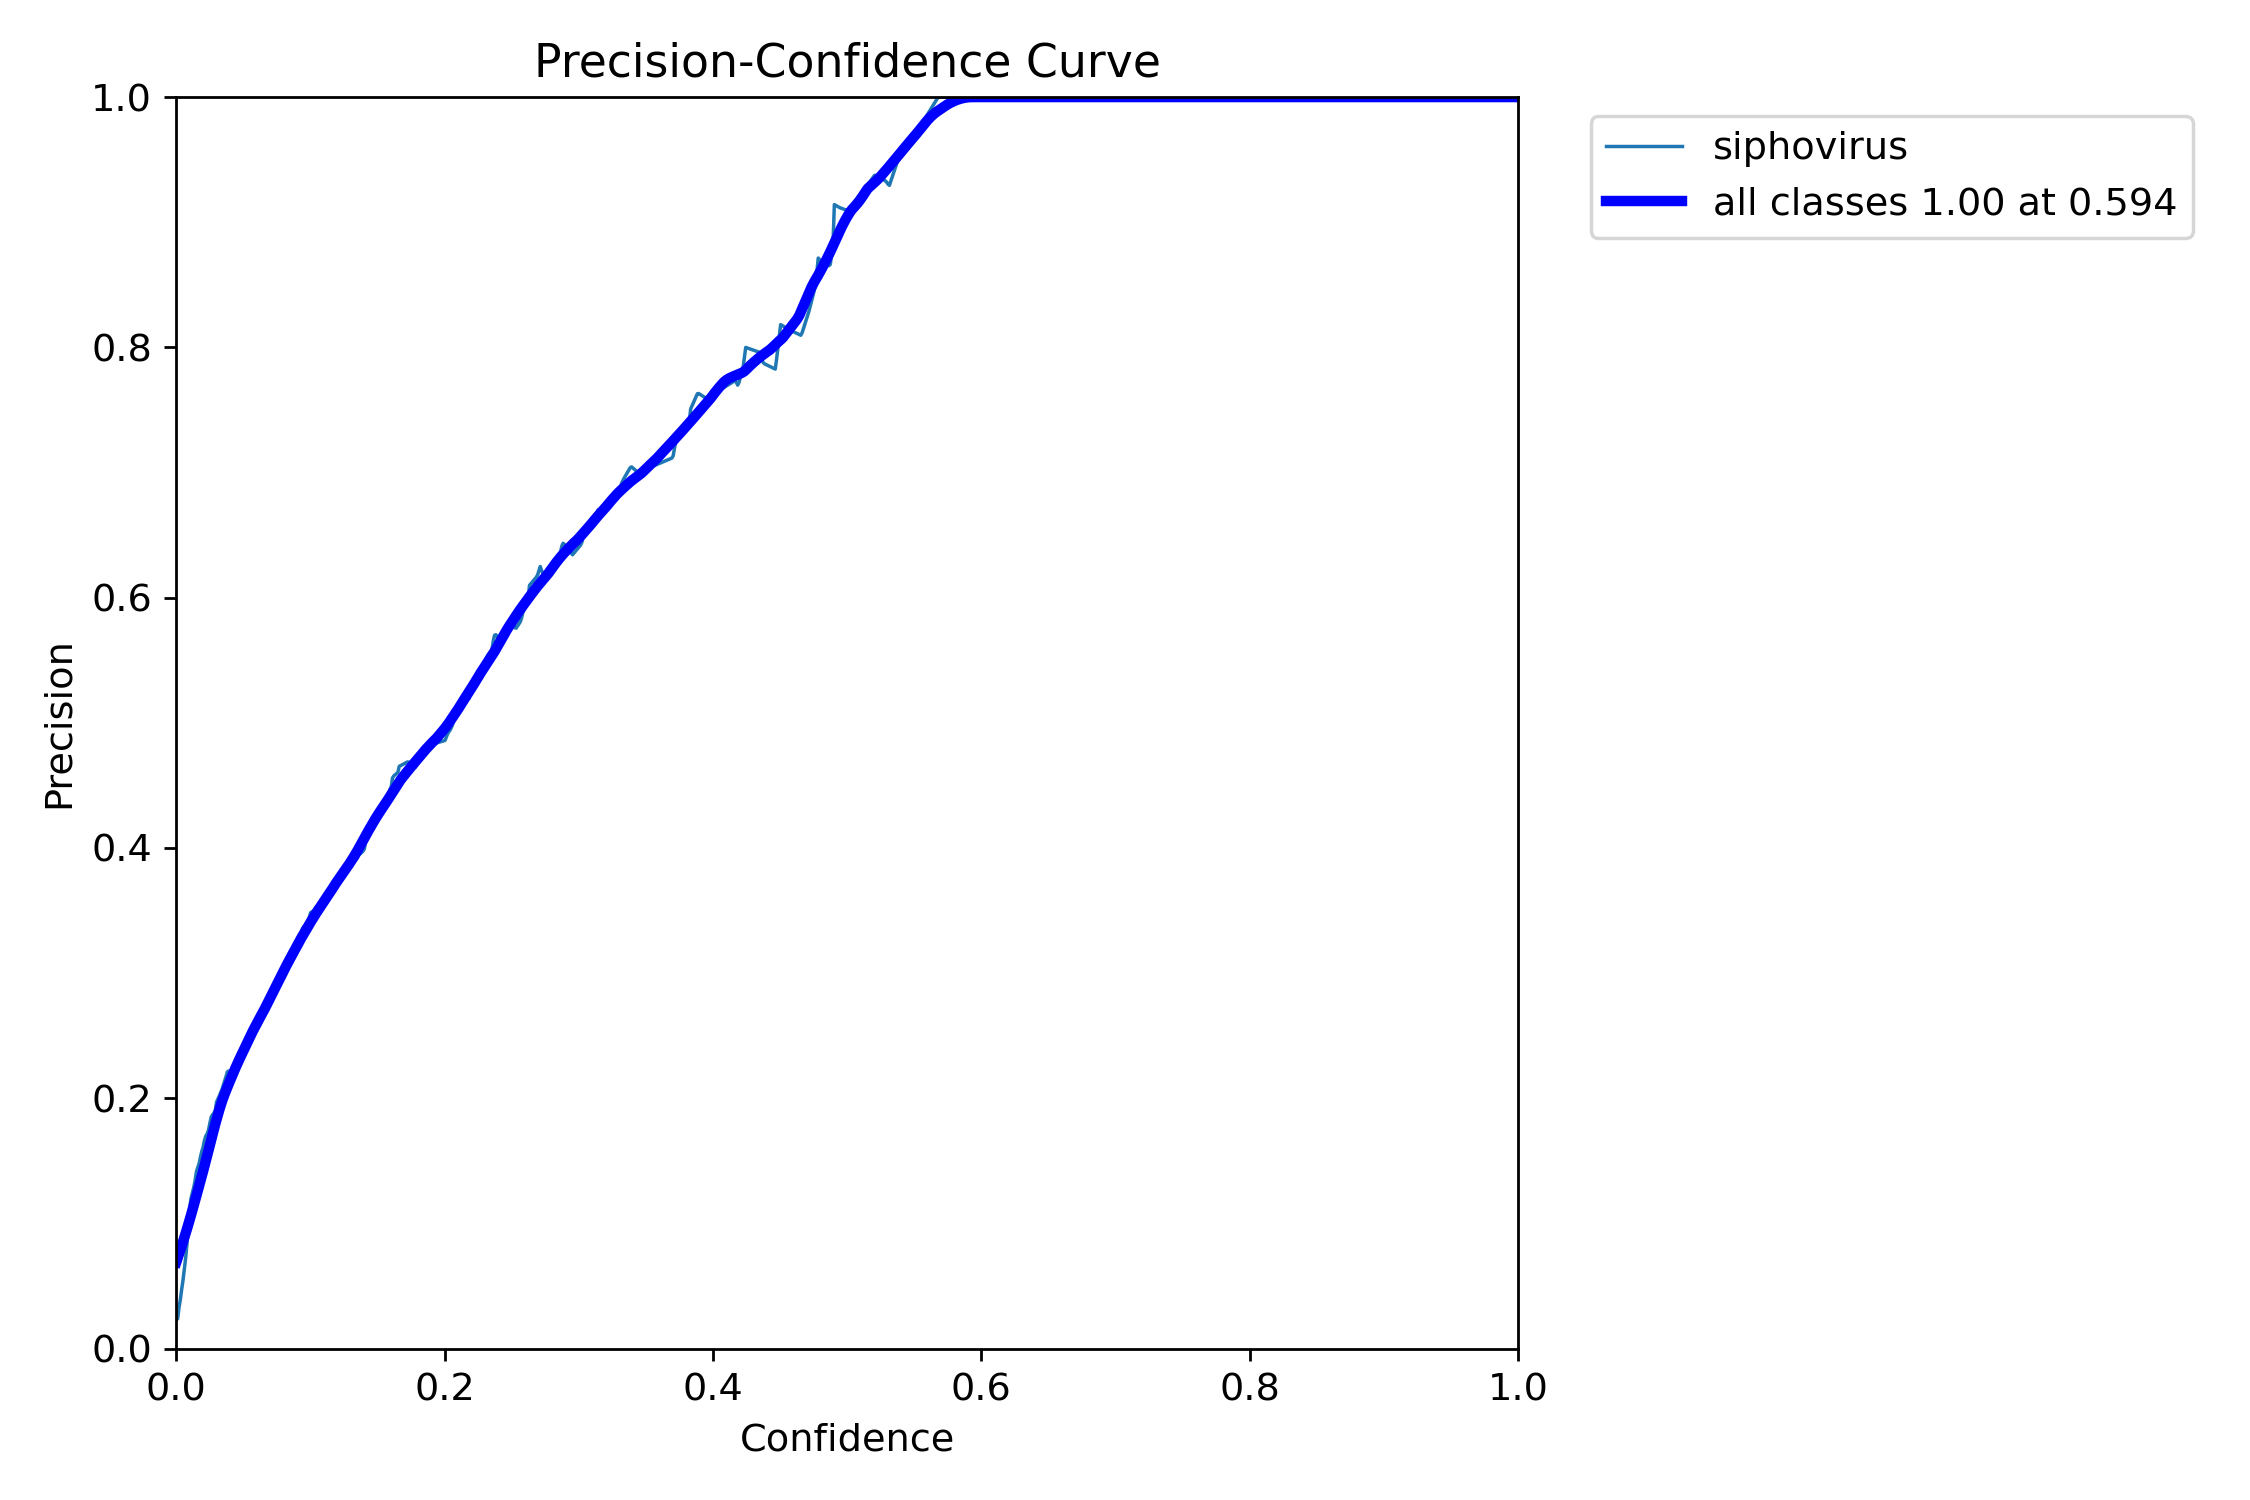
\includegraphics[height = 100px]{./figures/fig12b_50e_P_curve.png}
        \caption{Precision}
        \end{center}
    \end{subfigure}
    \hfill
    \begin{subfigure}[b]{0.25\textwidth}
    \begin{center}
        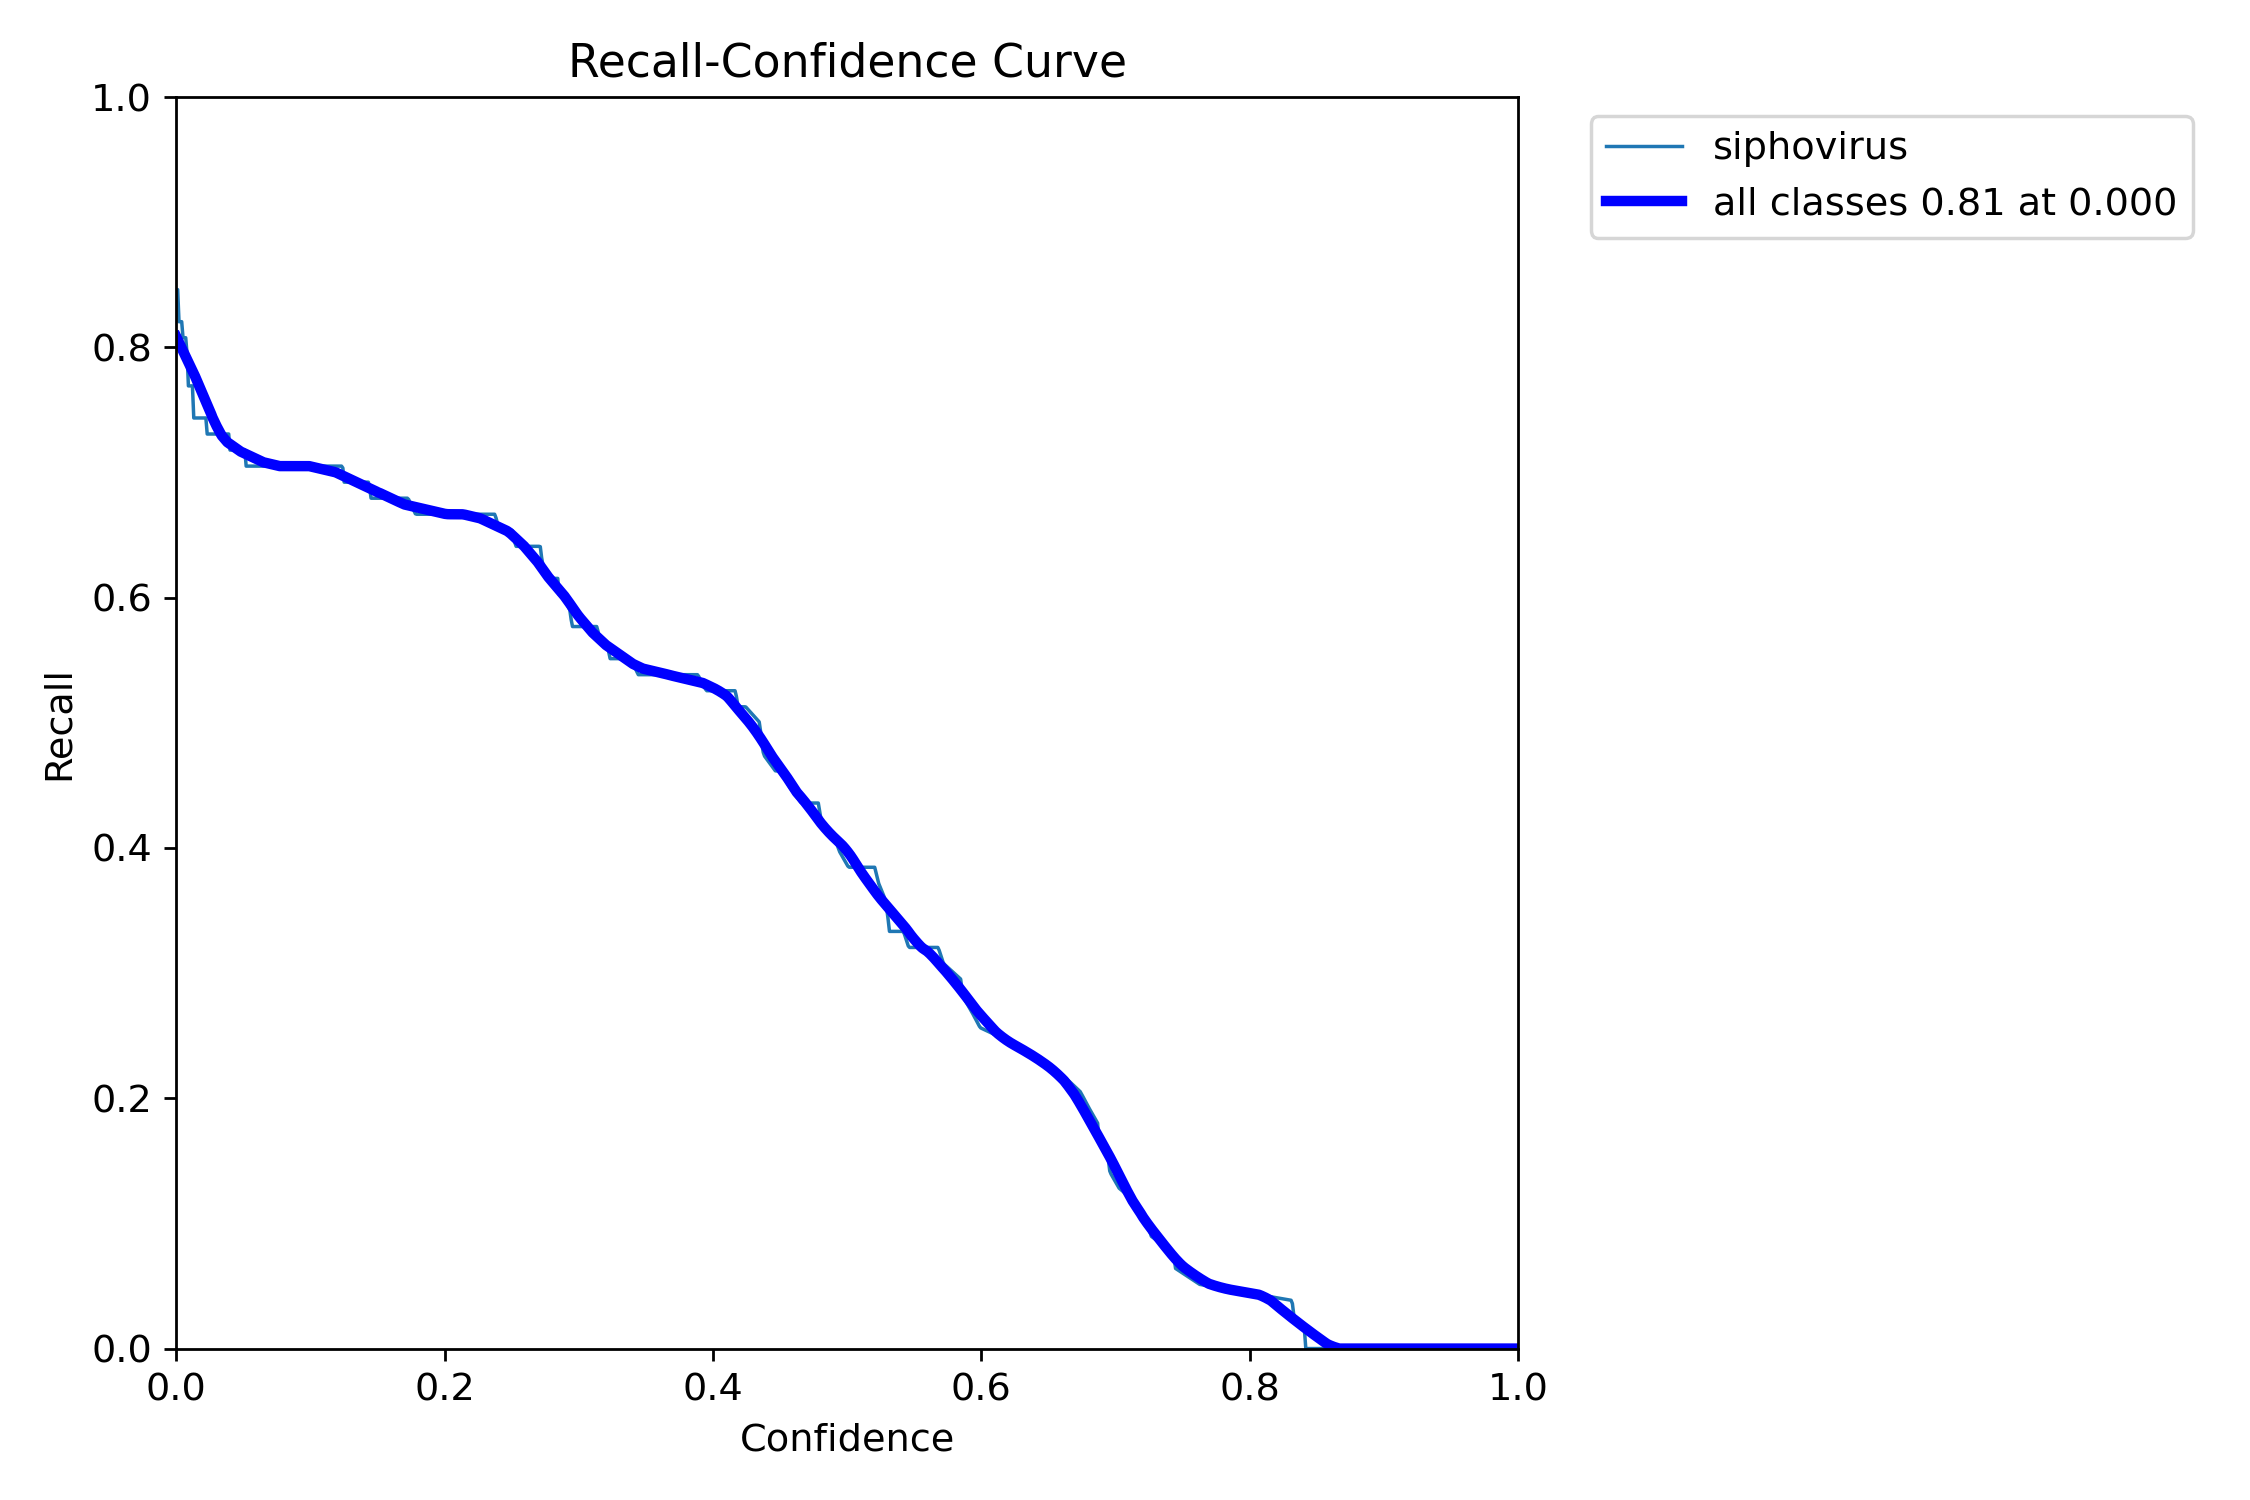
\includegraphics[height = 100px]{./figures/fig12c_50e_R_curve.png}
        \caption{Recall}
        \end{center}
    \end{subfigure}
    \caption{Performance metrics vs confidence threshold (50 epochs)}
    \label{fig12}
\end{figure}

By analyzing Figure \ref{fig13}, we observe these improvements in the form of an increased number of predictions across different scenarios and higher confidence levels for true positives. However, the model still misidentifies some objects as siphoviruses (as seen in the second image), underscoring the need to fine-tune hyperparameters and use a more diverse set of training images.

\begin{figure}[H]
\begin{center}
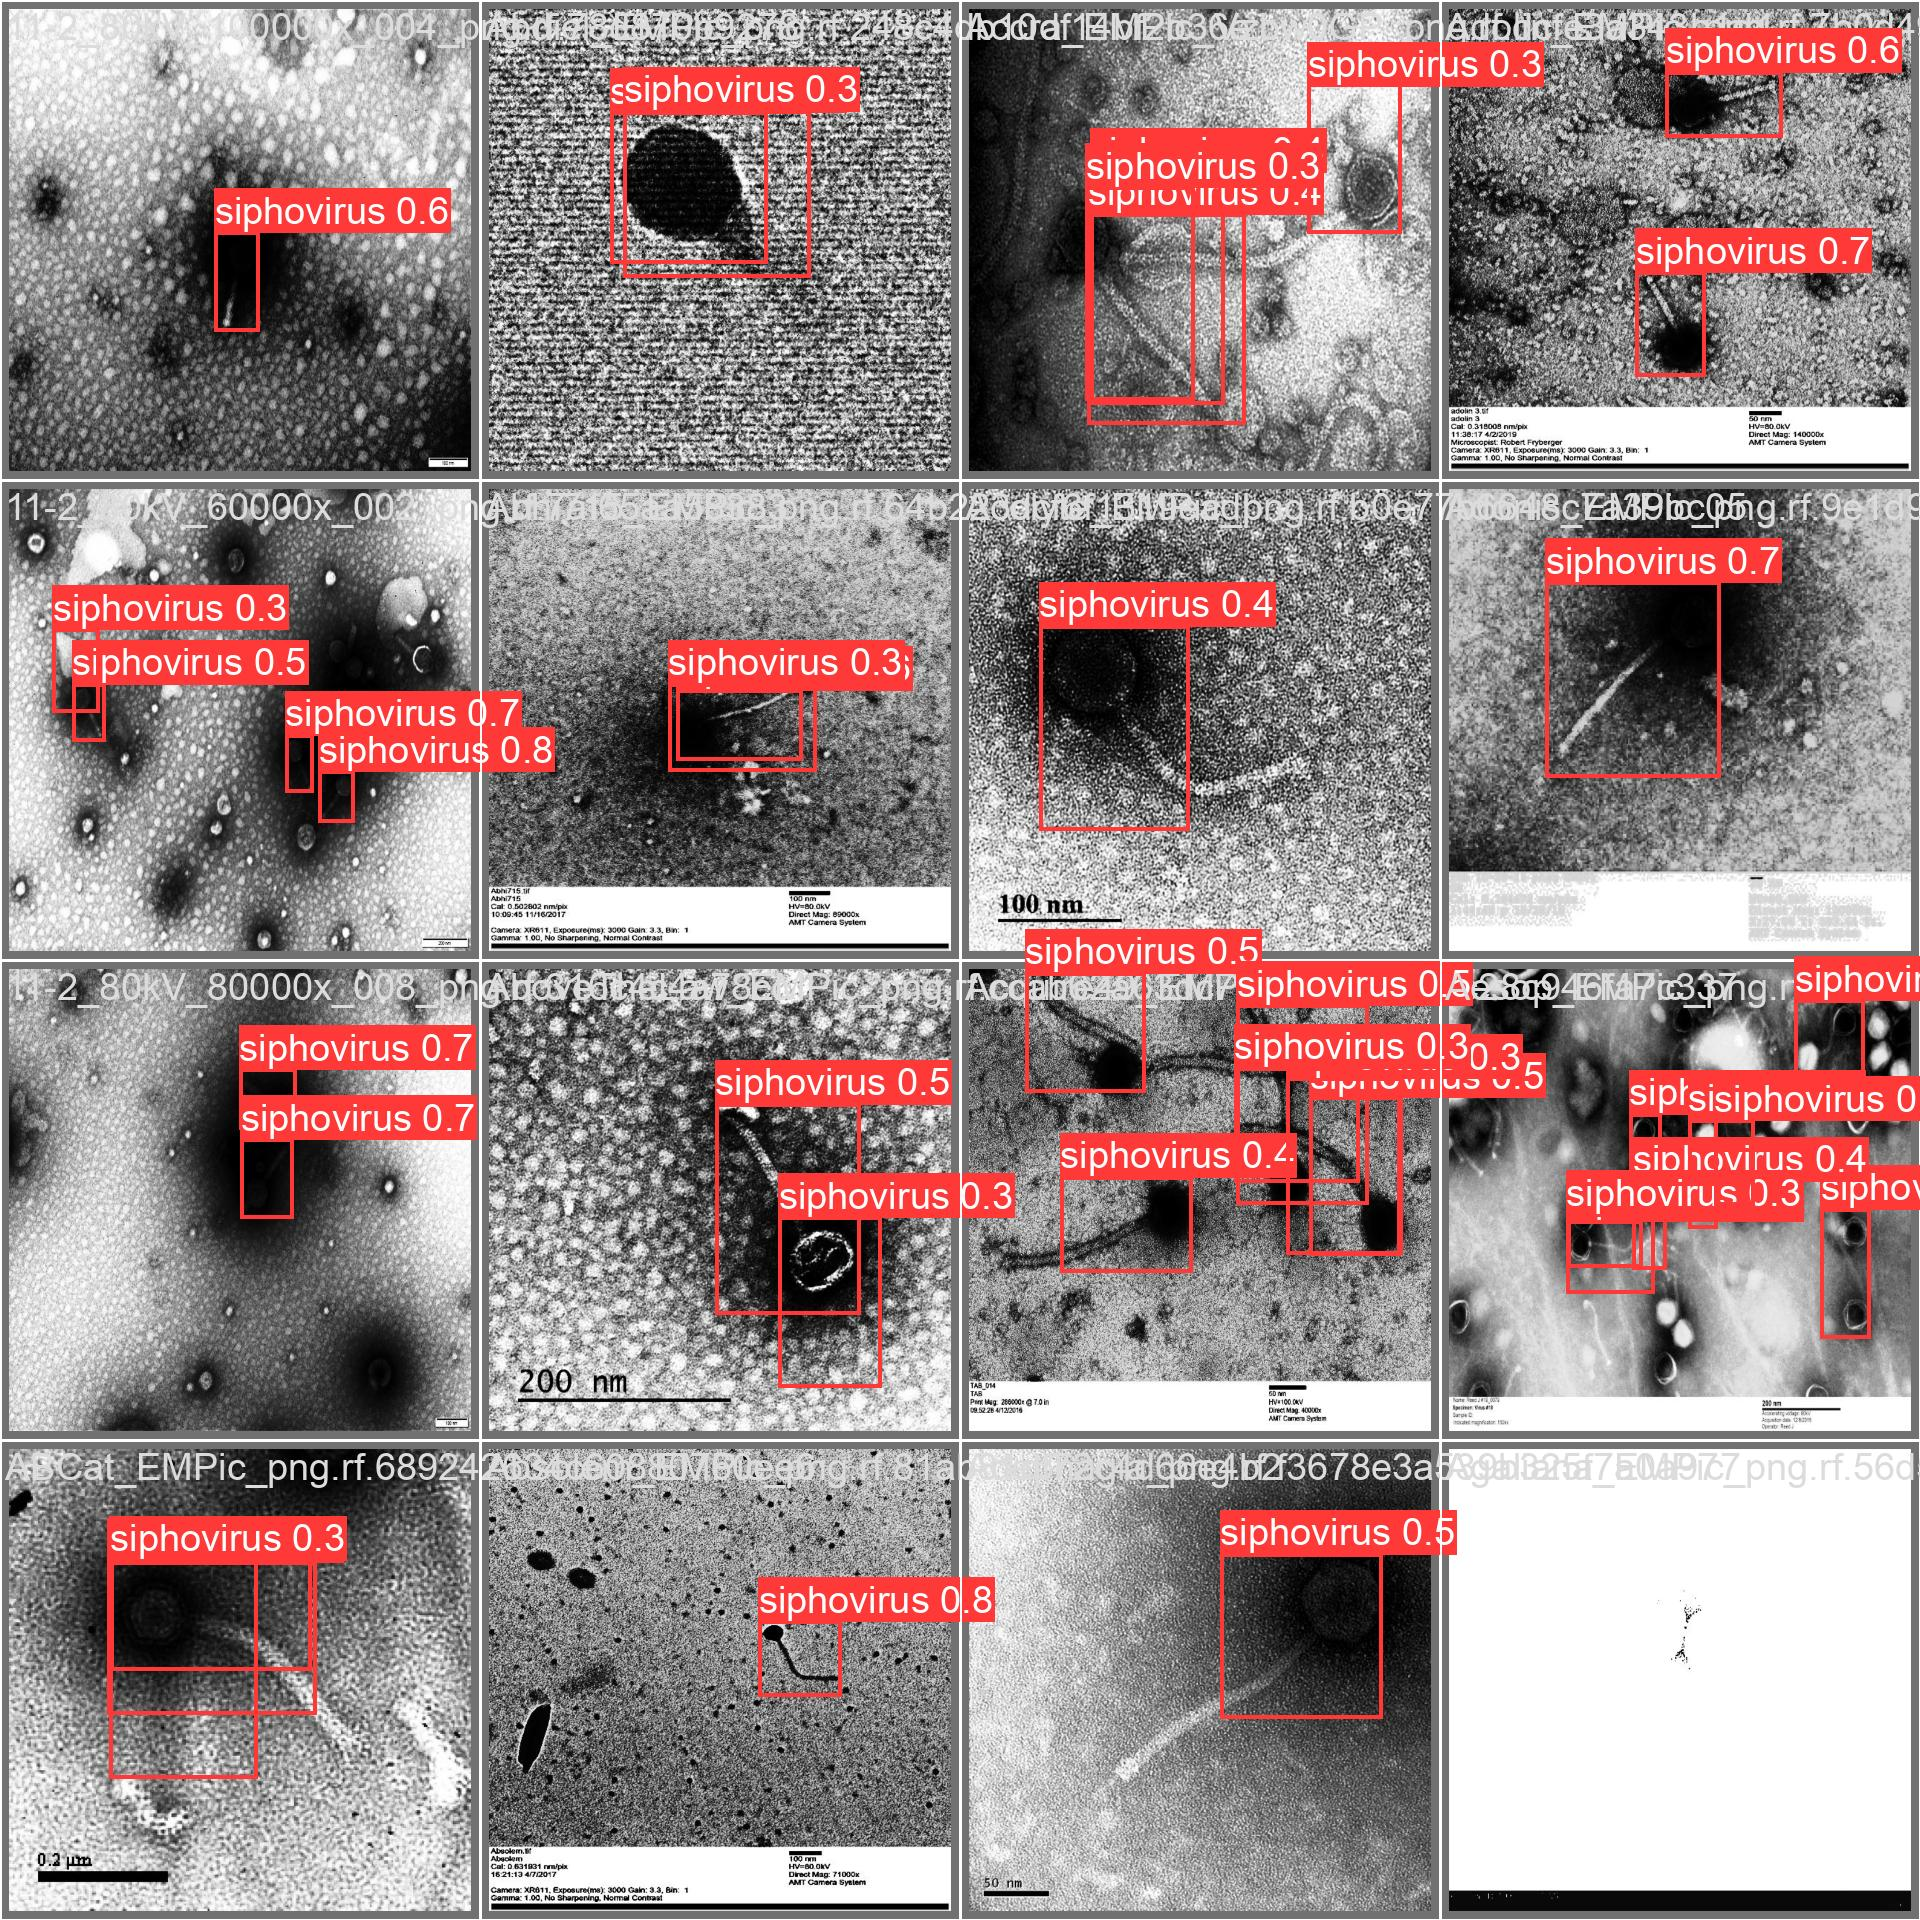
\includegraphics[width=.4\textwidth]{./figures/fig13_50e_val_batch0_pred.jpg}
\caption{Performance for validation batch - 50 epochs} \label{fig13}
\end{center}
\end{figure}

\section{Conclusions and Future Work} 
In this work we gave the first steps towards the development of a phage viral particle classifier using YOLO algorithms, having attained in this first iteration an encouraging F1 score of \textit{circa} 0.6 for a confidence threshold around 0.4 despite the occurrence of over-fitting and model conservativeness. 

The next steps in the PhageScan roadmap involve enhancing our dataset with greater diversity and incorporating additional classes for training. This initiative aims to fine-tune hyperparameters to achieve a minimum accuracy of 75\%, ensuring the model can accurately identify and differentiate between various virus types. 

Following this milestone, we plan to explore the implementation of automated measurements and feature identification techniques. This includes experimenting with methods such as OCR for scale identification and automated measurement, as well as edge contour detection for isolating features like tails and capsids. Ultimately, these efforts will enable us to estimate genome sizes based on these parameters, advancing our understanding and capabilities in virus characterization.

\newpage
%
% ---- Bibliography ----
%
% BibTeX users should specify bibliography style 'splncs04'.
% References will then be sorted and formatted in the correct style.
%
%\bibliographystyle{splncs04}
\bibliographystyle{unsrt}
\bibliography{bibliography}
%

\end{document}
